\documentclass[11pt, abstract=on, openany]{scrreprt}
\newenvironment{acknowledgements}{%
  \renewcommand{\abstractname}{Acknowledgements}%
  \begin{abstract}
}{%
  \end{abstract}
}

% % Setup page dimensions using the geometry package
\usepackage[a4paper, total={6.2in, 9.2in}]{geometry}


% Load essential packages
\usepackage{lipsum}          % Dummy text
\usepackage[utf8]{inputenc}  % Input encoding
\usepackage[T1]{fontenc}     % Font encoding
\usepackage[english]{babel}  % Language settings
\usepackage{lmodern}         % Modern LaTeX fonts
\usepackage{layout}          % Layout customization

% Using biblatex with IEEE style
\usepackage{csquotes}
\usepackage{scrhack}
\usepackage[backend=biber, style=numeric, sorting=none, maxbibnames=6, minbibnames=1]{biblatex}
\addbibresource{bibliography.bib}  % Link to your BibTeX database file

\usepackage{calc}


% Mathematical symbols and environments
\usepackage{amsmath, amsfonts, amssymb, mathrsfs}

\usepackage{changepage}

% Do not include the chapter in numbering
\usepackage{chngcntr}
\counterwithout{equation}{chapter}  % Detach equation counter from chapter
\counterwithout{figure}{chapter}    % Detach figure counter from chapter
\counterwithout{table}{chapter}     % Detach table counter from chapter

% Algorithms
\usepackage{algorithm}
\usepackage[table,xcdraw]{xcolor}
\usepackage[hang,flushmargin]{footmisc} 
\usepackage{booktabs}
\usepackage{bm,bbm}
\usepackage[noend]{algpseudocode}
\newcommand\Algphase[1]{%
\vspace*{-0.5\baselineskip}\Statex\hspace*{\dimexpr-\algorithmicindent-2pt\relax}\rule{0.9\textwidth}{0.4pt}%
\Statex\hspace*{-\algorithmicindent}\textbf{#1}%
\vspace*{-0.5\baselineskip}\Statex\hspace*{\dimexpr-\algorithmicindent-2pt\relax}\rule{0.9\textwidth}{0.4pt}%
}

\usepackage{multirow}
\usepackage{arydshln} % this causes problems with the superborder glossary style formatting
\dashlinegap=2pt

\usepackage{colortbl}
\usepackage{adjustbox}

% Graphics, figures, and subcaptions
\usepackage{graphicx}
\graphicspath{{img/}}        % Root directory for graphics
\usepackage{subcaption}      % Subfigures
\usepackage{float}           % Better float control
\usepackage{placeins}        % use \FloatBarrier to prevent floats (figures, tables, ...) from passing a specific point such as start of the next section
\usepackage{wrapfig}         % Wrapping text around figures

% PDF handling
\usepackage{pdfpages}

% caption formatting
\usepackage{caption}
\DeclareCaptionLabelSeparator{colon}{: }
\captionsetup{
    format=plain, % alignes multiline caption text with "Figure", "Table", etc. rather than with the beginning of the caption text
    %format=hang, % alignes multiline caption text with the beginning of the caption text
    labelsep=colon,
    labelformat=simple
}


% Header/footer customization
\usepackage[headsepline, footsepline, plainfootsepline]{scrlayer-scrpage}
\clearpairofpagestyles
\automark{chapter}
\ihead{\leftmark{}}
\ofoot[\thepage]{\thepage}



% Indentation and spacing
\setlength{\parindent}{0cm}  % No indentation at the beginning of paragraphs
\setlength{\parskip}{1em}    % Adjust space between paragraphs

% Notes and annotations
\usepackage[ngerman,linecolor=gray,bordercolor=gray,backgroundcolor=yellow]{todonotes}

% Code highlighting
\usepackage{listings}
\usepackage{color}
\definecolor{mygreen}{rgb}{0,0.6,0}
\definecolor{mymauve}{rgb}{0.58,0,0.82}
\lstset{
  basicstyle=\ttfamily,
  breaklines=true,
  captionpos=b,
  commentstyle=\color{mygreen},
  escapeinside={\%*}{*)},
  keywordstyle=\color{blue},
  stringstyle=\color{mymauve},
  frame=single,
  frameround=tttt
}

% Title, author, and date settings
\title{Prosodic Feature Modelling in Transformers for Speaker Verification}
\author{Fabian Bosshard, Andrin Fassbind}
\date{\today}
\makeatletter
\let\myTitle\@title
\makeatother

% Hyperlink settings
\usepackage[hidelinks, pdftex]{hyperref}
\hypersetup{
  pdftitle={\myTitle},
  pdfdisplaydoctitle=true,
  bookmarksnumbered,
  pdfstartview={FitH}
}

% Enumerated lists customization
\usepackage{enumitem}

% Diagrams and plots
% \usepackage{pgfplots, pgfplotstable, sfmath} %sfmath verändert die Schriftart in Formeln
\usepackage{pgfplots, pgfplotstable}
\pgfplotsset{compat=1.18} % adjust to your version
\usetikzlibrary{patterns, arrows, shapes, positioning, arrows.meta, calc, math, 3d, matrix}


% lengths

\newlength{\melwidth}
\newlength{\melheight}

\newlength{\imageheight}
\settoheight{\imageheight}{\includegraphics{spectrogram.pdf}}

\newlength{\imagewidth}
\settowidth{\imagewidth}{\includegraphics{spectrogram.pdf}}

\newlength{\halfimagewidth}
\setlength{\halfimagewidth}{0.5\imagewidth}





% Text formatting for bibliography
\usepackage{ragged2e}

% Acronym handling
\usepackage[nopostdot, nogroupskip, style=super, nonumberlist]{glossaries}
\setlength{\glsdescwidth}{0.8\textwidth}
\makeglossaries

\newacronym{ai}{AI}{artificial intelligence}
\newacronym{lm}{LM}{language model}
\newacronym{llm}{LLM}{large language model}
\newacronym{gpt}{GPT}{Generative Pre-trained Transformer}
\newacronym{rl}{RL}{reinforcement learning}
\newacronym{ml}{ML}{machine learning}
\newacronym{nlp}{NLP}{natural language processing}
\newacronym{xai}{XAI}{explainable artificial intelligence}
\newacronym{hmi}{HMI}{human-machine interaction}
\newacronym{sota}{SOTA}{state-of-the-art}
\newacronym{zhaw}{ZHAW}{Zurich University of Applied Sciences}

\newacronym{mlp}{MLP}{multilayer perceptron}
\newacronym{dnn}{DNN}{deep neural network}
\newacronym{cnn}{CNN}{convolutional neural network}
\newacronym{rnn}{RNN}{recurrent neural network}
\newacronym{lstm}{LSTM}{long short term memory}
\newacronym{blstm}{BLSTM}{bidirectional long short-term memory}
\newacronym{hmm}{HMM}{hidden Markov model}
\newacronym{gan}{GAN}{generative adversarial network}
\newacronym{resnet}{ResNet}{residual neural network}
\newacronym{ssast}{SSAST}{self-supervised audio spectrogram transformer}
\newacronym{vit}{ViT}{Vision Transformer}

\newacronym{sr}{SR}{speaker recognition}
\newacronym{sv}{SV}{speaker verification}
\newacronym{si}{SI}{speaker identification}
\newacronym{sc}{SC}{speaker clustering}
\newacronym{asr}{ASR}{automatic speech recognition}
\newacronym{far}{FAR}{false acceptance rate}
\newacronym{frr}{FRR}{false rejection rate}
\newacronym{eer}{EER}{equal error rate}
\newacronym{cer}{CER}{character error rate}
\newacronym{wer}{WER}{word error rate}
\newacronym{mr}{MR}{misclassification rate}
\newacronym{rer}{RER}{relative error rate}
\newacronym{mse}{MSE}{mean squared error}
\newacronym{infonce}{InfoNCE}{information noise-contrastive estimation}
\newacronym{adam}{Adam}{adaptive moment estimation}

\newacronym{fft}{FFT}{fast Fourier transform}
\newacronym{stft}{STFT}{short-time Fourier transform}
\newacronym{mfcc}{MFCC}{mel-frequency cepstral coefficient}
\newacronym{snr}{SNR}{signal-to-noise ratio}
\newacronym{sst}{SST}{supra-segmental temporal information}
\newacronym{fba}{FBA}{frame-based acoustic information}
\newacronym{os}{OS}{original segment}
\newacronym{ss}{SS}{shuffled within segment}
\newacronym{su}{SU}{shuffled within utterance}

\newacronym{ctc}{CTC}{connectionist temporal classification}
\newacronym{lpc}{LPC}{linear predictive coding}
\newacronym{cpc}{CPC}{contrastive predictive coding}
\newacronym{apc}{APC}{autoregressive predictive coding}
\newacronym{mhsa}{MHSA}{multi-head self-attention}

\newacronym{mo}{$\mathcal{M}_\text{o}$}{model pretrained on original spectrograms}
\newacronym{ms}{$\mathcal{M}_\text{s}$}{model pretrained on shuffled spectrograms}
\newacronym{moo}{$\mathcal{M}_\text{o/o}$}{model pretrained on original and finetuned on original spectrograms}
\newacronym{mos}{$\mathcal{M}_\text{o/s}$}{model pretrained on original and finetuned on shuffled spectrograms}
\newacronym{mso}{$\mathcal{M}_\text{s/o}$}{model pretrained on shuffled and finetuned on original spectrograms}
\newacronym{mss}{$\mathcal{M}_\text{s/s}$}{model pretrained on shuffled and finetuned on shuffled spectrograms}


\begin{document}

% Title page and originality declaration
\begin{titlepage}
\newcommand{\HRuleThick}{\rule{\linewidth}{0.6mm}} % Horizontal line command
\newcommand{\HRule}{\rule{\linewidth}{0.6mm}} % Horizontal line command

\centering

\includegraphics[width=8.6cm]{img/Logo_CAI/Druckaufloesung/A4-en-zhaw-cai-sw-ohne-byline.eps}\\[2.8cm]

\center % Center page content

\textsc{\large Bachelor's Thesis}\\[0.3cm] 

% Title Section
\makeatletter
\HRuleThick \\[0.3cm]
{\huge \bfseries \myTitle}\\[0.1cm]
\HRule \\[2.5cm]

% Change footnote symbol to a star
\renewcommand{\thefootnote}{\fnsymbol{footnote}}

% Author and Supervisor Section
\begin{minipage}[t]{0.4\textwidth}
\begin{flushleft} \large
\emph{Authors:}\\
Fabian Bosshard\footnotemark[1]\\
Andrin Fassbind\footnotemark[1]
\end{flushleft}
\end{minipage}
~
\begin{minipage}[t]{0.4\textwidth}
\begin{flushright} \large
\emph{Supervisor:} \\
Prof. Dr. Thilo Stadelmann\\
\end{flushright}
\end{minipage}\\[3.0cm]

% \begin{center} % Center the GitHub link
% \large{\url{https://github.com/???????????????}}\\[2cm]
% \end{center}


% Date Section
{\large \today}\\[2cm]

\footnotetext[1]{Equal contribution.}

% Reset footnote numbering and style if needed beyond this point
\renewcommand{\thefootnote}{\arabic{footnote}}
\setcounter{footnote}{0}

\end{titlepage}

\clearpage
\pagestyle{empty} % Disable page numbers
% Logo positioned absolutely
\begin{tikzpicture}[remember picture, overlay]
    \node[anchor=north west, inner sep=0pt] at (current page.north west)[xshift=1.5cm, yshift=-2cm]{
        
\includegraphics[width=6cm]{img/Logo_SoE/Druck/CMYK/de-soe-cmyk.eps}
    };
\end{tikzpicture}


\vspace{3.5cm}

% Title
\begin{center}
    {\Large\textbf{DECLARATION OF ORIGINALITY}}\\[0.2cm]
    \textbf{Bachelor’s Thesis at the School of Engineering}
\end{center}

\vspace{1cm}

By submitting this Bachelor's thesis, the undersigned student confirms that this thesis is their own work and was written without the help of a third party. (Group works: the performance of the other group members is not considered as a third party).

The student declares that all sources in the text (including Internet pages) and appendices have been correctly disclosed. This means that there has been no plagiarism, i.e., no sections of the Bachelor's thesis have been partially or wholly taken from other texts and represented as the student’s own work or included without being correctly referenced.

\textcolor{red}{Any misconduct will be dealt with according to paragraphs 39 and 40 of the General Academic Regulations for Bachelor's and Master's Degree courses at the Zurich University of Applied Sciences (Rahmenprüfungsordnung ZHAW (RPO)) and subject to the provisions for disciplinary action stipulated in the University regulations.}



\vspace{2.7cm}

% City, Date and Name of Student
\begin{minipage}[t]{0.48\textwidth}
    Date:\\[0.7cm]
    ...................................................................
\end{minipage}
\hfill
\begin{minipage}[t]{0.48\textwidth}
    Signature:\\[0.7cm]
    ...................................................................\\[0.7cm]
    ...................................................................
\end{minipage}

% Signature images positioned with TikZ
\begin{tikzpicture}[remember picture, overlay]
    % Adjust the 'xshift' and 'yshift' to position your first signature
    \node[anchor=south, inner sep=0pt] at (current page.north east)[xshift=-8.6cm, yshift=-21.3cm]{
        \includegraphics[width=3.6cm]{img/signature_fabian.png}
    };
    % Adjust the 'xshift' and 'yshift' to position your second signature
    \node[anchor=south, inner sep=0pt] at (current page.north east)[xshift=-8.7cm, yshift=-22.65cm]{
        \includegraphics[width=4.5cm]{img/signature_andrin.png}
    };
    % Adjust the 'xshift' and 'yshift' to position your second signature
    \node[anchor=south, inner sep=0pt] at (current page.north east)[xshift=-16.2cm, yshift=-21.3cm]{
        
\includegraphics[width=4.7cm]{img/date_thesis.png}
    };
\end{tikzpicture}


% Small text positioned absolutely at the bottom
\begin{tikzpicture}[remember picture, overlay]
    \node[anchor=south west, inner sep=0pt] at (current page.south west)[xshift=1.5cm, yshift=2cm]{
        
\includegraphics[width=2cm]{img/Logo_SoE/cmyk_byline_e.eps}
    };
\end{tikzpicture}
\clearpage

% Abstract and acknowledgements
\selectlanguage{english}
\begin{abstract}
% Abstract
% - [typical architecture: ca. 1-2 sentences for each of motivation; problem statement; approach; results; relevency of results]

Recent advancements in \gls{sv} technologies, particularly through \glspl{dnn}, have significantly contributed to the field of \gls{sr}. However, despite these advancements, challenges persist, particularly in terms of robustness in noisy environments and the effective modeling of \gls{sst} — attributes such as intonation and stress, which play a crucial role in human speaker recognition capabilities.

This thesis investigates the effectiveness of transformer models, a type of \glspl{dnn} known for their success in \glspl{llm} like ChatGPT, in capturing these \gls{sst} for \gls{sv} tasks. We hypothesize that by pre-training transformer models to reconstruct hidden frames in speech spectrograms, the temporal nuances essential for accurate speaker recognition can be better captured. Our approach includes the development of a transformer-based \gls{sv} system that is pre-trained on a task that is expected to capture these \gls{sst} and subsequently fine-tuned on \gls{sv}.

Initial experiments demonstrate that models trained on shuffled spectrograms, where temporal information is deliberately obscured, surprisingly do not show the expected decrease in performance. This suggests that these models may not rely on \gls{sst} as significantly as hypothesized and are capable of achieving robust \gls{sv} by predominantly learning from \gls{fba}, contrary to initial expectations.

The findings of this research could potentially improve the understanding of the dependencies of \glspl{dnn} on temporal versus spectral features in \gls{sv} tasks and contribute to the development of more robust \gls{sv} systems capable of performing accurately under varied acoustic conditions.

\glsresetall % Reset all glossary entries to ensure they are fully expanded at first use in the main document.

\end{abstract}

\begin{acknowledgements}
We would like to thank our supervisor, Prof. Dr. Thilo Stadelmann, for his excellent guidance throughout our bachelor thesis. His respect for our ideas and his encouragement significantly contributed to our approach to research. Prof. Stadelmann's readiness to answer our queries and his conceptual guidance were fundamental to our work.

We are grateful to Dr. Marc André Stadelmann for his assistance in setting up the necessary infrastructure at the Centre for Artificial Intelligence, which provided us with access to their advanced GPU cluster. His help was crucial for the effective implementation of our project and significantly enhanced our research capabilities.

We would also like to thank Dr. Yuan Gong and his colleagues from the Massachusetts Institute of Technology for publicly releasing the code of their research, answering questions about it as well as sharing detailed performance logs with us. Dr. Gong's responsiveness and openness in discussing implementation details were very valuable to our project.

Special thanks to Daniel Neururer for his advice on optimizing data loading processes, which helped us deepen our understanding of practical data handling in machine learning environments.

Lastly, we thank our families and friends for their support throughout this journey.
\end{acknowledgements}

% Roman numbering for initial pages
\pagestyle{plain} 
\pagenumbering{roman}
\tableofcontents
\clearpage

% Abbreviations
\printglossary[type=\acronymtype, title=List of Abbreviations]
\clearpage

% Arabic numbering for main content
\pagenumbering{arabic}
\chapter{Introduction}
\label{chapter:introduction}
% 1. Introduction
% - Motivation [understandable also for a general audience]
% - Problem statement [formulation of research question]
% (- Own contributions [novelties you claim as your own])
% (- Organization of thesis [brief description of how the remaining chapters are organized])


\section{Motivation}\label{sec:motivation}
\label{motivation}

\Gls{sv} is a biometric process used to verify the identity of a speaker based on their voice characteristics. It differs from \gls{si}, which involves identifying a speaker among a group. In \gls{sv}, the system compares the incoming speech data against another speech recording of a claimed identity to confirm whether the claim is true. Essentially, the task is binary - confirming or denying the identity claim - making it particularly suitable for access control and authentication purposes. \Gls{sv} and \gls{si} are subtasks of the broader field \gls{sr} \cite{kinnunen2006realtime}. Figure \ref{fig:difference_sv_si} shows the difference between the two tasks.

\begin{figure}[h]
    \centering
    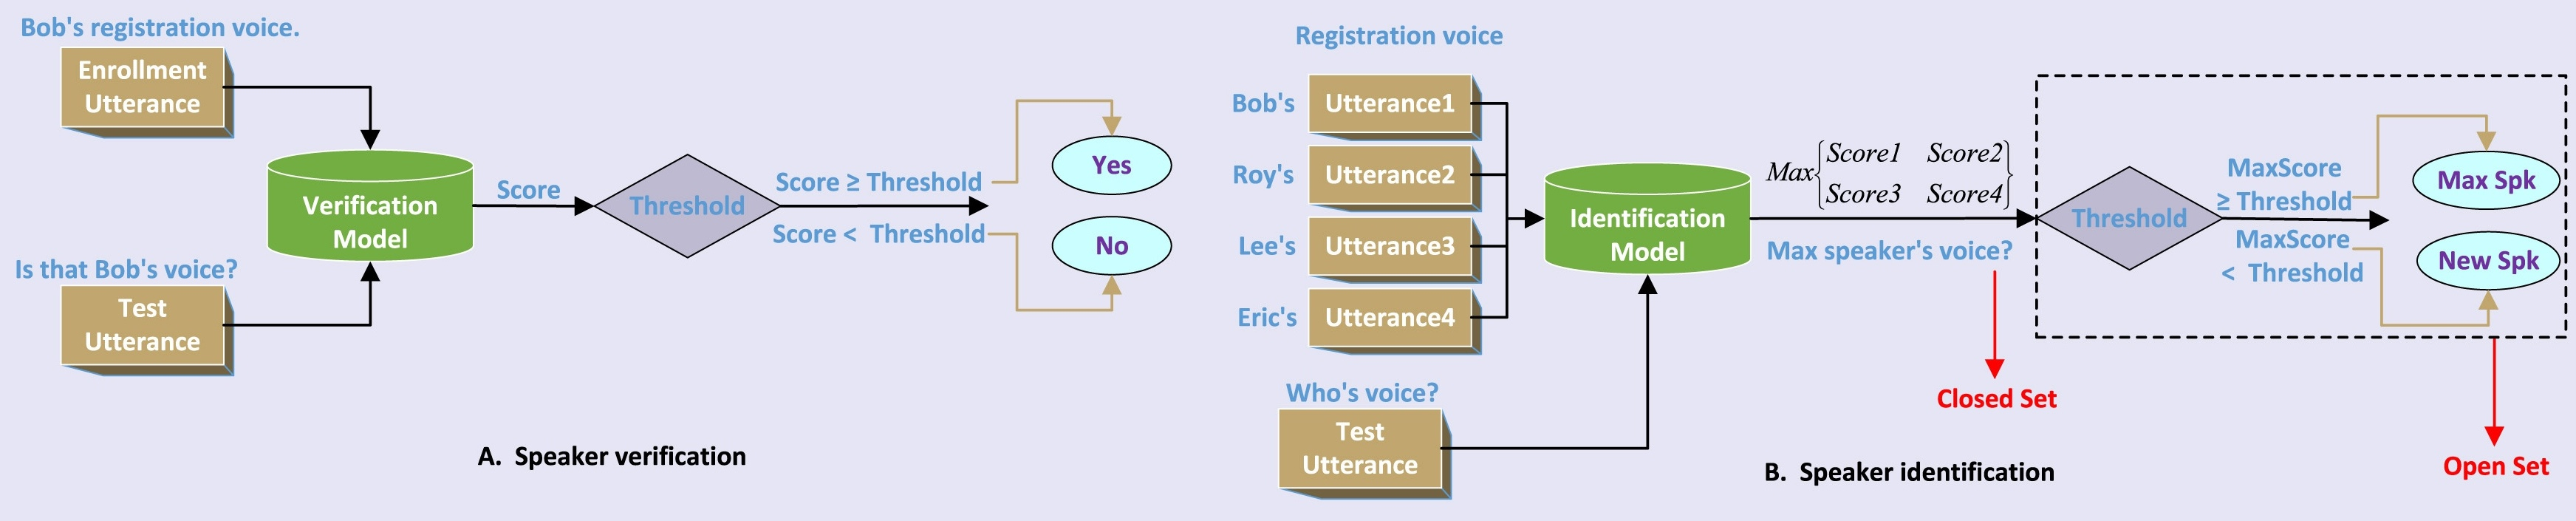
\includegraphics[width=\textwidth]{img/speaker_identification_verification.jpg}
    \caption{Difference between speaker verification and identification. Image from \cite{bai2021speaker}.}
    \label{fig:difference_sv_si}
\end{figure}

With the proliferation of smart devices and voice-activated interfaces such as Siri, Cortana, and Alexa, \gls{sv} has become an indispensable technology in ensuring secure and personalized user experiences. These systems rely on the unique characteristics of a user's voice to confirm their identity, enabling tasks ranging from sending messages to making purchases. Despite significant advancements, automatic \gls{sv} systems still face challenges, particularly in noisy or unpredictable environments, where they often struggle to maintain accuracy and reliability \cites{khazaleh2024investigation, sun2023noise}.

Humans excel in recognizing speakers even in adverse conditions, a skill partly attributable to their adeptness at interpreting prosodic features - subtle variations in rhythm, stress, and intonation that convey important information about the speaker's identity \cites{rose2002forensic, hansen2015speaker}. Similarly, enhancing the capability of machines to understand and utilize these prosodic cues could markedly improve \gls{sv} systems, especially in challenging scenarios \cite{stadelmann2009unfolding}. Henceforth, we refer to this type of information as \gls{sst}, which is distinguished from \gls{fba}, referring to short-term spectral information. % fba is short-term spectral information only in machines? 

\Glspl{dnn} have become very good at \gls{sv} \cite{huh2023voxsrc}. It was therefore often assumed that, similar to humans, they are now able to make use of \gls{sst} as well \cites{stadelmann2018capturing, zhao2020improving, ye2021deep}. However, recent research shows that at least for some architectures, such as \glspl{cnn}, \glspl{rnn}, and \glspl{resnet} this hypothesis needs to be rejected. Specifically it was found that for the aforementioned models, when trained on manipulated data that does not contain any \gls{sst} anymore, the performance does not decrease as expected, but stays the same or sometimes even increases \cite{neururer2023deep}. This "\textit{deep cheating}" phenomenon is significant as it suggests a potential path to improving the performance, reliability and robustness of \gls{sv} systems.

This leads us to question whether a different architectural approach could surmount these obstacles. Consequently, this thesis proposes the exploration of transformers \cite{vaswani2017attention}, renowned for their effectiveness in sequence-based tasks and potential for modeling complex dependencies over time. By investigating these models' ability to utilize \gls{sst}, we aim to uncover whether they can enhance the accuracy and robustness of \gls{sv} systems.


\section{Problem Statement}

This thesis aims to investigate the modeling of \gls{sst} in transformer models, a type of neural network architecture for example associated with \glspl{llm} like ChatGPT. By pre-training these models to reconstruct hidden frames in speech spectrograms, it is hypothesized that they can better capture the temporal nuances of speech, leading to improved \gls{sv} accuracy, overall through enhanced capturing of supra-segmental features.

To test these assertions, experiments are conducted with transformers focusing on the capture of \gls{sst}. Performance comparisons are made between models trained on original speech data and those trained on manipulated data devoid of any temporal information. The outcomes of these experiments will help assess the efficacy of transformers in \gls{sv} tasks and their ability to robustly model essential speech characteristics.


\section{Contributions}

While not achieving state-of-the-art, we can show that for the transformer architecture (at least when using the configuration described in chapter \ref{chapter:methods}) the same oddity holds true as for the other architectures tested in \cite{neururer2023deep}. Specifically, training with data that includes \gls{sst} does not improve \gls{sv} performance; on the contrary, it actually has a detrimental impact on the latter.


\section{Organization}\label{sec:organization}

The rest of this thesis is organized into four chapters and two appendices:

\begin{itemize}
    \item \textbf{Chapter \ref{chapter:foundation}: Foundations} covers foundational concepts related to \gls{sv} on a high level. It also reviews the related work this thesis builds upon.
    \item \textbf{Chapter \ref{chapter:methods}: Methods} contains a detailed description of the methodologies employed in this thesis, focusing on data preprocessing as well as pretraining and finetuning of the model.
    \item \textbf{Chapter \ref{chapter:results}: Results} presents the results of the conducted experiments as well as a discussion thereof. The pretraining results are presented and the tendency of transformers, when finetuned for \gls{sv}, to model \gls{sst} is discussed.
    \item \textbf{Chapter \ref{chapter:conclusion}: Conclusion} summarizes the findings of the thesis and discusses their implications for future research in \gls{sv}.
    \item \textbf{Appendix \ref{appendix_resynth}: Resynthesizing Audio from Spectrograms} describes a problem we encountered when resynthesizing audio from spectrograms and the solution we came up with to mitigate it.
    \item \textbf{Appendix \ref{appendix_resynth_examples}: More Resynthesized Spectrograms} contains additional resynthesized spectrograms that were developed during our project.
\end{itemize}
\pagebreak [3]


\section{Implementation}\label{sec:implementation}
The code developed for this project is publicly available at the following URL:\\ \href{https://github.com/Ironmomo/SpeakerVerificationBA}{https://github.com/Ironmomo/SpeakerVerificationBA}.
























% In recent years, advancements in automatic speaker recognition technology have been notable, mainly due to the development of deep learning methods \cite{brown2022voxsrc, huh2023voxsrc}. However, these systems still struggle to match human performance, especially in challenging conditions like background noise or with short utterances from unknown speakers. Research at \gls{zhaw} has identified a significant gap in how \glspl{dnn} comprehend and use speaker-specific traits such as \gls{sst} in \gls{sr} \cite{neururer2023deep}.

% Existing literature emphasizes the importance of speaker-specific traits and the ability of \glspl{dnn} to learn them. Yet, studies show that current \glspl{cnn}, \glspl{rnn}, and \glspl{resnet} used for \gls{sv} and \gls{sc} often overlook these traits when trained on clean datasets. This phenomenon, termed "\textit{deep cheating}" is significant as it suggests a potential path to improving related tasks and reducing error rates.




% The objectives of the thesis include:
% \begin{itemize}

% \item Conducting a thorough review of relevant literature and previous studies to identify existing approaches and gaps in research.
% \item Collaboratively devising a clear approach, guided by supervisors, including defining the architecture and training methods for transformer models.
% \item Setting up the necessary infrastructure for data collection and processing, including local setups and GPU resources.
% \item Developing and refining a prototype of the transformer-based speaker recognition system through innovative experimentation.
% \item Ultimately, presenting a scholarly document outlining the motivation, methodology, evaluations, and findings of the research, emphasizing the advancements in speaker recognition achieved through transformer models.
% \end{itemize}

% This thesis aims to contribute meaningfully to the ongoing discussion on voice recognition while addressing the current limitations of automatic speaker recognition systems.
















\chapter{Foundations}
\label{chapter:foundation}
% 2. Foundations
% - [Introduction of foundations not generally known to professionals in computer science]
% - Related work [similar to respective chapters in papers: review the relevant related work by briefly summarizing it incl.used methods and achieved results, and then contrasting it with own task, i.e., show any gaps to own problem statement]


\section{Representation of Audio Signals}

In \gls{sr} systems, audio signals are typically represented as sequences of feature vectors. Various methods exist to represent these features, each providing different insights into the audio signal's characteristics and properties.

\subsection{Raw Waveform}
The raw waveform of an audio signal represents the scaled voltage amplitude of the sound wave as it varies over time. This waveform is essentially a direct digital encoding of the air pressure variations caused by sound waves. It is captured through a process of analog-to-digital conversion where the continuous sound wave is sampled at regular intervals (sampling rate) and quantized into digital values.

This representation is one of the most fundamental forms of audio data, providing a time-domain view where each sample point represents the amplitude of the audio signal at a given instant. The sampling rate, typically measured in kilohertz, defines the number of samples captured per second and is crucial in determining the quality and range of frequencies that can be accurately represented in the digital waveform.

More details on the analog-to-digital conversion process can be found in \cite{lyons2010understanding} or \cite{oppenheim1996signals}.

A raw waveform can be written as \({s} \in \mathbb{R}^l\), where \({s}[n]\) denotes the amplitude of the \(n\)-th sample, and \(l\) is the total number of samples. The sampling frequency \(f_s\), an important parameter in the analog-to-digital conversion process, dictates the temporal resolution of the waveform. The Nyquist-Shannon sampling theorem states that \(f_s\) should be at least twice the maximum frequency component present in the audio signal to adequately capture its frequency content without aliasing \cite{Nyquist1928, Shannon1949}.

In audio processing and \gls{sr} systems, the raw waveform often serves as the basis for further transformations and feature extraction methods, which transform the time-domain data into formats more suitable for various analyses and machine learning applications.

\subsection{Mel Spectogram}

Another representation method is a spectrogram, where the frequency composition ($y$-axis) of the signal is shown as it varies over time ($x$-axis). A variation of the spectrogram is the Mel spectrogram, in which each frequency of the audio signal is logarithmically scaled to better account for human perception of different frequency bands. The representation as a (Mel) spectrogram offers the advantage of a visual capture of the audio signal. Therefore, image processing models like the neural networks described in Section \ref{motivation} can be used for the algorithmic processing of audio in this representation. For the rest of this thesis, we treat the Mel spectrogram as a matrix $X$ with $M$ rows and $L$ columns, where $X[i]$ denotes the $i^{\text{th}}$ column/frame in the spectrogram:
\begin{equation}
\label{eq:spectrogram_matrixz}
    X =
    \begin{bmatrix}
    \vert & \vert & \vert & \vert & \vert &       & \vert  \\
    X[0]  & X[1]  & X[2]  & X[3]  & X[4]  &\cdots & X[L-1] \\
    \vert & \vert & \vert & \vert & \vert &       & \vert
    \end{bmatrix}
    \in \mathbb{R}^{M \times L}
\end{equation}

Figure \ref{waveform_spectrogram} shows the raw waveform of one sample of the pretraining dataset and its corresponding Mel spectrogram. More details on the conversion of time-domain signals to Mel spectrograms can be found in section \ref{sec:mel_spectrogram_conversion}.

\begin{figure}[h]
    \centering
    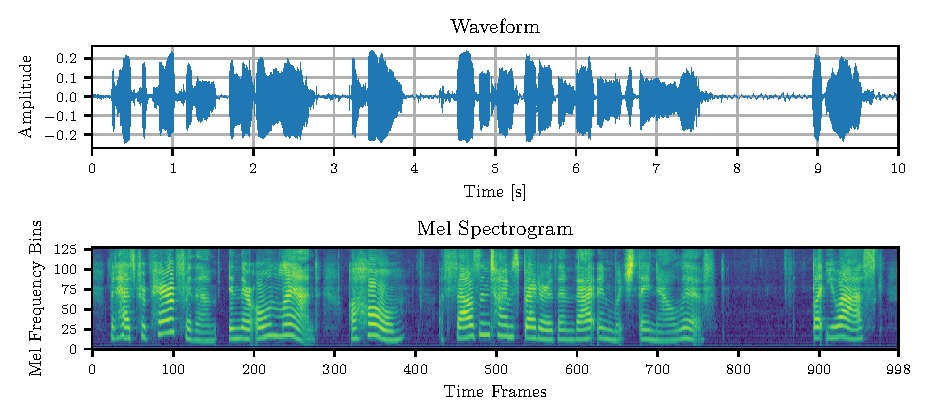
\includegraphics[width=1.0\linewidth]{img/plots/waveform_spectrogram.pdf}
    \caption{Raw waveform signal (top) and the corresponding mel spectrogram (bottom).}
    \label{waveform_spectrogram}
\end{figure}


\section{Linguistic Characteristics in the Context of Speaker Recognition}
\label{sec:spectroinformation}

To better understand the challenges in modeling prosodic features for \gls{sr}, a detailed analysis of linguistic peculiarities is required. Humans have exceptional abilities in identifying speakers and sub-tasks of \gls{sr} such as \gls{sv}. Linguistics has intensively dealt with this topic and has gained important insights. In particular, it has been shown that spectro-temporal acoustic-phonetic information is crucial for the high performance of the human brain in \gls{sr} \cites{rose2002forensic, hansen2015speaker}.

% \subsection{Spectro-temporal Acoustic-Phonetic Information in Language}\label{sec:spectroinformation}
% 1 subsectin wo die einzig isch inere section sött mer glaub vermide

\textit{Spectro-temporal acoustic-phonetic information} refers to the combination of spectral (frequency-related) and temporal (time-related) properties of speech signals. Spectral information includes the distribution of energy across various frequency bands of the speech signal. This can be used to identify features such as formants, which represent characteristic resonance frequencies in human speech. Formants manifest as peaks in the spectrum and enable the identification of characteristic frequency patterns associated with certain vowels \cite{small1998phonetics}. This is shown in Figure~\ref{fig:formants}.

\begin{figure}[h]
\begin{subfigure}[b]{0.47\textwidth}
   \centering
   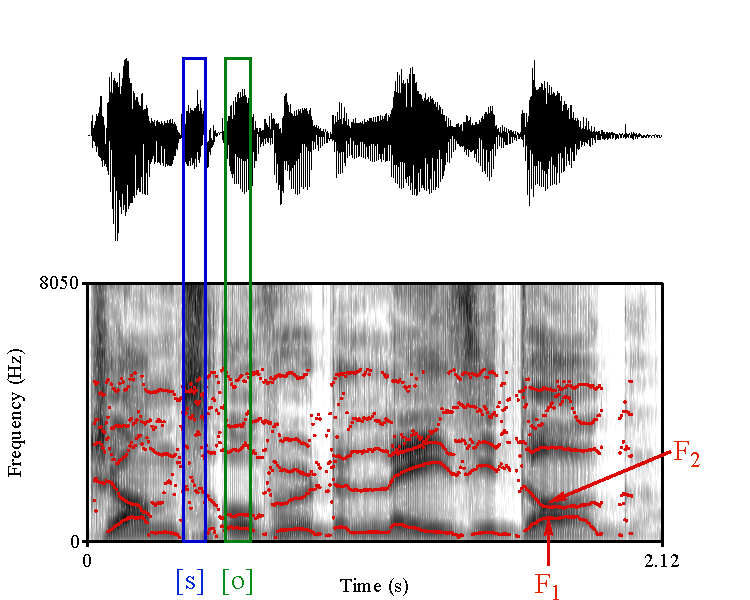
\includegraphics[width=1\textwidth]{img/english-sound-segment-nice3.pdf}
\end{subfigure}%
\begin{subfigure}[b]{0.53\textwidth}
   \centering
   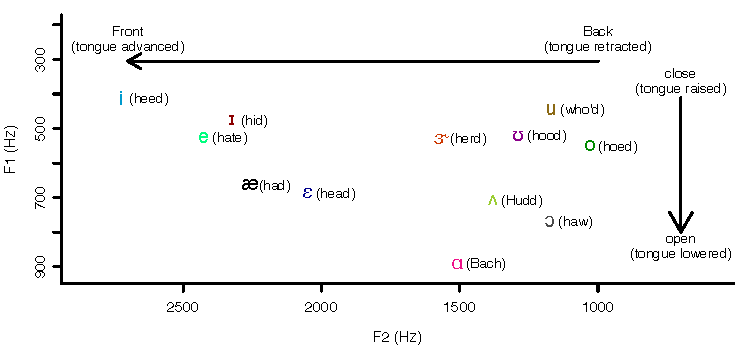
\includegraphics[width=1\textwidth]{img/AllvowelsH95--formants-raw--mean.pdf}
\end{subfigure}
\caption{Raw waveform and corresponding spectrogram of a speech recording (left); average vowel formants in the $F_1,F_2$ vowel space over a set of 139 speakers (right). Image from \cite{tavakoli2024statistics}.}
\label{fig:formants}
\end{figure}

Temporal information refers to the sequence of sound events in the speech signal, characterized by features such as stress patterns, speaking rate, and intonation patterns. Stress patterns describe the emphasis of certain syllables, while speaking rate indicates the number of sounds or words per unit of time. Intonation describes the melody and pitch of the language.

The combination of these spectral and temporal information allows for the capture and analysis of complex linguistic features, which is crucial for automatic speech recognition, speech synthesis, and other speech processing applications. In phonetics, it is generally recognized that these features are unique and can thus be assigned to an individual speaker.


\section{Audio Signal Processing Using DNNs}

The basic approach to \gls{sr} using \glspl{dnn} is works as follows.
The voice recording is transformed into a suitable format. Often, this is a Mel spectrogram, as information not relevant to human perception is filtered out from the audio signal. This reduction in information content can be justified because humans excel in \gls{sr}, thus the audio information perceivable by the human auditory organ should also be sufficient for a \gls{dnn}.

% \subsection{Frame-based Acoustic Information - \gls{fba}}

The audio signal is then divided into overlapping time windows, which serve as input for the \gls{dnn}. These windows typically have a length in the range of several tens of milliseconds. This approach offers several advantages: By using segments of the audio signal, the amount of data is reduced, leading to simpler models with lower dimensionality and shorter training time. Moreover, this method makes the model more robust against environmental noise, as it learns local features. These local features contain, as described in section \ref{sec:spectroinformation}, spectral information \gls{fba}. However, research points out that \gls{sst} plays a significant role in human \gls{sr} \cite{stadelmann2009unfolding}. To what extent \gls{dnn} consider \gls{sst} is discussed in \cite{neururer2023deep}.

\section{Quantifying the Utilization of SST}
\label{foundation_sst}

The mentioned paper, \cite{neururer2023deep}, represents the first systematic approach to investigate the modeling of \gls{sst} in \gls{dnn}. This section explains the method developed by the authors, which forms the basis and motivation for the present work.

The goal is to investigate whether state-of-the-art \gls{dnn}, when removing the \gls{sst} from the spectrogram inputs, are still able to achieve good performance in \gls{sr} tasks. If this is the case, it can at least be argued that \gls{dnn} are capable of compensating for the loss of \gls{sst} and therefore do not necessarily rely on them, but can instead rely on the remaining \gls{fba}.

To remove the \gls{sst} from the spectrogram while preserving the \gls{fba}, two approaches have been pursued:
\vspace{-\parskip}
\begin{itemize}[topsep=0.5\parskip, itemsep=0.0\parskip, parsep=0.5\parskip]
    \item \textbf{\gls{ss}}: The spectrogram is divided into equal-sized segments, within which the data is swapped on the time axis. %\glsunset{ss}
    \item \textbf{\gls{su}}: The spectrogram is also divided into equal-sized segments, but the data is swapped on the time axis before segmenting. %\glsunset{su}
\end{itemize}

Figure \ref{shuffle_sst_exploitation} illustrates the described process of swapping spectrogram information.

\begin{figure}[H]
\centering
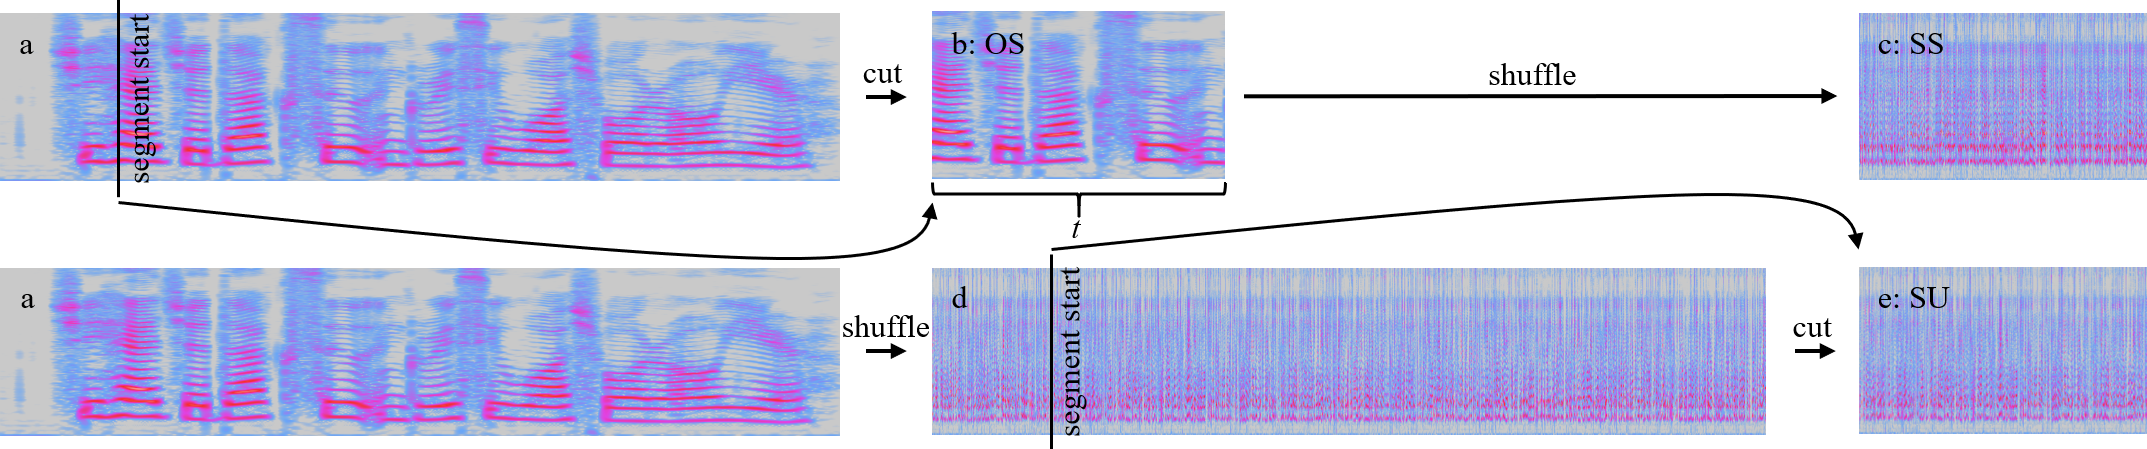
\includegraphics[width=1.0\linewidth]{img/segment-drawing.png}
\caption{Generation and shuffling of segments (image from \cite{neururer2023deep}).}
\label{shuffle_sst_exploitation}
\end{figure}

In \cite{neururer2023deep}, various \gls{dnn} models for \gls{sr} are tested on different training and evaluation datasets. This includes training on \gls{os} and evaluation on \gls{os}, \gls{ss}, and \gls{su} as well as training on \gls{ss} and evaluation on \gls{os}, \gls{ss}, and \gls{su}, and training on \gls{su} and evaluation on \gls{os}, \gls{ss}, and \gls{su}. The evaluated architectures include a \gls{cnn}, a \gls{rnn}, a \gls{resnet} and the F-\gls{resnet}. The results of these experiments are shown in Table \ref{sst_exploitation_results}.

In particular, the results show that training and evaluation on swapped data (SS/SS and SU/SU) deliver state-of-the-art performance in \gls{sc} and \gls{sv}, although the model does not utilize \gls{sst}. These results cast significant doubts on whether \glspl{dnn} actually learn \gls{sst} or whether they rely exclusively on \gls{fba} features \cite{neururer2023deep}.

If the performance of training and evaluation on the shuffled data were significantly lower than the performance of training and evaluation on the original data, it could be stated that the model relies on both \gls{fba} and \gls{sst}. 

The present thesis therefore investigates the performance of Transformers in \gls{sv} tasks and tries to determine whether they rely on \gls{sst}.

\newcommand{\OrigSeg}{OS}
\newcommand{\ShuffleSeg}{SS}
\newcommand{\ShuffleUtterance}{SU}

\newcommand{\markcell}[1]{\scriptsize{#1}$\Downarrow$\footnotesize}
\setlength{\tabcolsep}{2pt} % for the horizontal padding

\begin{table}[H]
	\centering
     \caption{Test results as reported in \cite{neururer2023deep} using original and shuffled spectrograms from the TIMIT dataset using four different \glspl{dnn}. \Gls{sc} performance (left) is measured using the \gls{mr} ($\mu/\sigma$) and \gls{sv} performance (right) is measured using the \gls{eer} ($\mu/\sigma$). Bold font indicates best results per model, cell coloring scales with quality per model.}
    %\begin{adjustbox}{width=\textwidth}
    	\begin{tabular}{ll|rrr|rrr}
    		\hline
    	 \multicolumn{2}{c|}{task $\rightarrow$}
    		 & \multicolumn{3}{c|}{Speaker Clustering}
    		 & \multicolumn{3}{c}{Speaker Verification} \\

    		 \multicolumn{2}{c|}{\scriptsize{training $\downarrow$ / test $\rightarrow$}}
    		 & \multicolumn{1}{c}{\OrigSeg}
    		 & \multicolumn{1}{c}{\ShuffleUtterance}
    		 & \multicolumn{1}{c|}{\ShuffleSeg}
    		 & \multicolumn{1}{c}{\OrigSeg}
    		 & \multicolumn{1}{c}{\ShuffleUtterance}
    		 & \multicolumn{1}{c}{\ShuffleSeg} \\ 
            \hline
    		\multirow{3}{*}{CNN \cite{lukic2017learning}}
    		 & \OrigSeg
    		 & \cellcolor[RGB]{0, 255, 0} \textbf{0.00 \scriptsize{$\sigma$0.00}}
    		 & \cellcolor[RGB]{255, 0, 0} 9.75 \scriptsize{$\sigma$0.94}
    		 & \cellcolor[RGB]{255, 39, 0} 9.00 \scriptsize{$\sigma$2.15}
    		 & \cellcolor[RGB]{80, 255, 0} 6.38 \scriptsize{$\sigma$0.12}
    		 & \cellcolor[RGB]{255, 0, 0} 12.02 \scriptsize{$\sigma$0.51}
    		 & \cellcolor[RGB]{255, 9, 0} 11.90 \scriptsize{$\sigma$0.46} \\
    		 & \ShuffleUtterance
    		 & \cellcolor[RGB]{255, 65, 0} 8.50 \scriptsize{$\sigma$2.42}
    		 & \cellcolor[RGB]{26, 255, 0} 0.50 \scriptsize{$\sigma$0.61}
    		 & \cellcolor[RGB]{91, 255, 0} 1.75 \scriptsize{$\sigma$0.61}
    		 & \cellcolor[RGB]{245, 255, 0} 8.55 \scriptsize{$\sigma$0.49}
    		 & \cellcolor[RGB]{16, 255, 0} 5.55 \scriptsize{$\sigma$0.06}
    		 & \cellcolor[RGB]{60, 255, 0} 6.12 \scriptsize{$\sigma$0.12} \\
    		 & \ShuffleSeg
    		 & \cellcolor[RGB]{255, 39, 0} 9.00 \scriptsize{$\sigma$1.66}
    		 & \cellcolor[RGB]{52, 255, 0} 1.00 \scriptsize{$\sigma$0.50}
    		 & \cellcolor[RGB]{65, 255, 0} 1.25 \scriptsize{$\sigma$0.00}
    		 & \cellcolor[RGB]{215, 255, 0} 8.16 \scriptsize{$\sigma$0.42}
    		 & \cellcolor[RGB]{0, 255, 0} \textbf{5.33 \scriptsize{$\sigma$0.18}}
    		 & \cellcolor[RGB]{34, 255, 0} 5.78 \scriptsize{$\sigma$0.16} \\
    		\hline
    		\multirow{3}{*}{RNN \cite{stadelmann2018capturing}}
    		 & \OrigSeg
    		 & \cellcolor[RGB]{170, 255, 0} 1.25 \scriptsize{$\sigma$1.12}
    		 & \cellcolor[RGB]{255, 136, 0} 2.75 \scriptsize{$\sigma$0.94}
    		 & \cellcolor[RGB]{255, 135, 0} 2.75 \scriptsize{$\sigma$0.50}
    		 & \cellcolor[RGB]{0, 255, 0} \textbf{3.53 \scriptsize{$\sigma$0.07}}
    		 & \cellcolor[RGB]{255, 0, 0} 4.19 \scriptsize{$\sigma$0.09}
    		 & \cellcolor[RGB]{255, 224, 0} 3.90 \scriptsize{$\sigma$0.12} \\
    		 & \ShuffleUtterance
    		 & \cellcolor[RGB]{255, 0, 0} 3.75 \scriptsize{$\sigma$1.37}
    		 & \cellcolor[RGB]{0, 255, 0} \textbf{0.00 \scriptsize{$\sigma$0.00}}
    		 & \cellcolor[RGB]{255, 169, 0} 2.50 \scriptsize{$\sigma$1.58}
    		 & \cellcolor[RGB]{255, 149, 0} 3.99 \scriptsize{$\sigma$0.16}
    		 & \cellcolor[RGB]{189, 255, 0} 3.78 \scriptsize{$\sigma$0.10}
    		 & \cellcolor[RGB]{97, 255, 0} 3.66 \scriptsize{$\sigma$0.13} \\
    		 & \ShuffleSeg
    		 & \cellcolor[RGB]{255, 238, 0} 2.00 \scriptsize{$\sigma$1.00}
    		 & \cellcolor[RGB]{170, 255, 0} 1.25 \scriptsize{$\sigma$0.79}
    		 & \cellcolor[RGB]{33, 255, 0} 0.25 \scriptsize{$\sigma$0.50}
    		 & \cellcolor[RGB]{255, 144, 0} 4.00 \scriptsize{$\sigma$0.07}
    		 & \cellcolor[RGB]{255, 232, 0} 3.89 \scriptsize{$\sigma$0.06}
    		 & \cellcolor[RGB]{4, 255, 0} 3.54 \scriptsize{$\sigma$0.05} \\
    		\hline
    		\multirow{3}{*}{ResNet \cite{xie2019utterance}}
    		 & \OrigSeg
    		 & \cellcolor[RGB]{0, 255, 0} \textbf{1.00 \scriptsize{$\sigma$0.94}}
    		 & \cellcolor[RGB]{255, 157, 0} 8.25 \scriptsize{$\sigma$4.78}
    		 & \cellcolor[RGB]{255, 0, 0} 11.50 \scriptsize{$\sigma$4.29}
    		 & \cellcolor[RGB]{0, 255, 0} \textbf{4.96 \scriptsize{$\sigma$0.19}}
    		 & \cellcolor[RGB]{255, 0, 0} 10.34 \scriptsize{$\sigma$1.56}
    		 & \cellcolor[RGB]{255, 106, 0} 9.21 \scriptsize{$\sigma$1.15} \\
    		 & \ShuffleUtterance
    		 & \cellcolor[RGB]{72, 255, 0} 2.50 \scriptsize{$\sigma$1.77}
    		 & \cellcolor[RGB]{0, 255, 0} \textbf{1.00 \scriptsize{$\sigma$0.50}}
    		 & \cellcolor[RGB]{97, 255, 0} 3.00 \scriptsize{$\sigma$1.27}
    		 & \cellcolor[RGB]{154, 255, 0} 6.59 \scriptsize{$\sigma$0.25}
    		 & \cellcolor[RGB]{122, 255, 0} 6.25 \scriptsize{$\sigma$0.23}
    		 & \cellcolor[RGB]{133, 255, 0} 6.37 \scriptsize{$\sigma$0.35} \\
    		 & \ShuffleSeg
    		 & \cellcolor[RGB]{84, 255, 0} 2.75 \scriptsize{$\sigma$0.94}
    		 & \cellcolor[RGB]{12, 255, 0} 1.25 \scriptsize{$\sigma$1.12}
    		 & \cellcolor[RGB]{0, 255, 0} \textbf{1.00 \scriptsize{$\sigma$0.94}}
    		 & \cellcolor[RGB]{87, 255, 0} 5.89 \scriptsize{$\sigma$0.25}
    		 & \cellcolor[RGB]{108, 255, 0} 6.11 \scriptsize{$\sigma$0.31}
    		 & \cellcolor[RGB]{79, 255, 0} 5.80 \scriptsize{$\sigma$0.11} \\
    		\hline
    		\multirow{3}{*}{F-ResNet \cite{chung2020in}}
    		 & \OrigSeg
    		 & \cellcolor[RGB]{117, 255, 0} 11.50 \scriptsize{$\sigma$2.15}
    		 & \cellcolor[RGB]{255, 0, 0} 37.50 \scriptsize{$\sigma$4.18}
    		 & \cellcolor[RGB]{255, 57, 0} 33.75 \scriptsize{$\sigma$4.18}
    		 & \cellcolor[RGB]{114, 255, 0} 12.20 \scriptsize{$\sigma$0.25}
    		 & \cellcolor[RGB]{255, 0, 0} 23.41 \scriptsize{$\sigma$1.73}
    		 & \cellcolor[RGB]{255, 104, 0} 20.47 \scriptsize{$\sigma$1.50} \\
    		 & \ShuffleUtterance
    		 & \cellcolor[RGB]{192, 255, 0} 16.50 \scriptsize{$\sigma$2.42}
    		 & \cellcolor[RGB]{30, 255, 0} 5.75 \scriptsize{$\sigma$1.70}
    		 & \cellcolor[RGB]{7, 255, 0} 4.25 \scriptsize{$\sigma$1.00}
    		 & \cellcolor[RGB]{217, 255, 0} 15.12 \scriptsize{$\sigma$0.84}
    		 & \cellcolor[RGB]{53, 255, 0} 10.46 \scriptsize{$\sigma$0.28}
    		 & \cellcolor[RGB]{26, 255, 0} 9.69 \scriptsize{$\sigma$0.20} \\
    		 & \ShuffleSeg
    		 & \cellcolor[RGB]{178, 255, 0} 15.50 \scriptsize{$\sigma$2.57}
    		 & \cellcolor[RGB]{45, 255, 0} 6.75 \scriptsize{$\sigma$1.50}
    		 & \cellcolor[RGB]{0, 255, 0} \textbf{3.75 \scriptsize{$\sigma$0.79}}
    		 & \cellcolor[RGB]{246, 255, 0} 15.91 \scriptsize{$\sigma$0.90}
    		 & \cellcolor[RGB]{32, 255, 0} 9.86 \scriptsize{$\sigma$0.11}
    		 & \cellcolor[RGB]{0, 255, 0} \textbf{8.95 \scriptsize{$\sigma$0.13}} \\
    		\hline
    	\end{tabular}
    %\end{adjustbox}
    \label{sst_exploitation_results}
\end{table}


\section{Contrastive Loss}
Contrastive loss is a metric learning technique widely used in machine learning to measure the similarity between pairs of data points. The idea of contrastive loss is to ensure that similar data points (positive pairs) are closer in an embedding space, while dissimilar data points (negative pairs) are farther apart. 

Contrastive loss was introduced in the context of Siamese networks, where the goal is to learn a function that maps input data into an embedding space where the similarity between data points can be easily measured \cite{Hadsell2006DimensionalityRB}. For \gls{sv}, it means that intra-speaker embeddings are closer in the embedding space while inter-speaker embeddings are farther apart. The contrastive loss function is described in \ref{methods_contrastive_loss}.



















% \section{Sprachliche Besonderheiten im Kontext der Sprechererkennung}

% Um die Herausforderungen bei der Modellierung prosodischer Merkmale für die Sprechererkennung (SV) besser zu verstehen, ist eine eingehende Analyse der Sprachbesonderheiten erforderlich. Der Mensch verfügt über außergewöhnliche Fähigkeiten bei der Identifizierung von Sprechern und deren Teilaufgaben wie der Sprecherüberprüfung (Speaker Verification). Die Linguistik hat sich intensiv mit dieser Thematik befasst und dabei wichtige Erkenntnisse gewonnen. Insbesondere hat sich gezeigt, dass spektro-temporale akustisch-phonetische Informationen für die hohe Leistungsfähigkeit des menschlichen Gehirns in der Sprechererkennung entscheidend sind \cites{rose2002forensic, hansen2015speaker}.

% \subsection{Spektro-temporale akustisch-phonetische Informationen in der Sprache}\label{sec:spectroinformation}

% \textit{Spektro-zeitliche akustisch-phonetische Informationen} beziehen sich auf die Kombination spektraler (frequenzbezogener) und zeitlicher Eigenschaften von Sprachsignalen. Spektrale Informationen umfassen die Verteilung der Energie in verschiedenen Frequenzbereichen des Sprachsignals. Diese können zur Identifizierung von Merkmalen wie Formanten genutzt werden, die charakteristische Resonanzfrequenzen in der menschlichen Sprache repräsentieren. Formanten manifestieren sich als Peaks im Spektrum und ermöglichen die Identifizierung charakteristischer Resonanzfrequenzen, die bestimmten Vokalen zugeordnet werden können \cite{small1998phonetics}.

% Zeitliche Informationen beziehen sich auf die Abfolge von Schallereignissen im Sprachsignal, die durch Merkmale wie Betonungsmuster (Stress Pattern), Sprechgeschwindigkeit (Speaking Rate) und Intonationsmuster gekennzeichnet sind. Betonungsmuster beschreiben die Hervorhebung bestimmter Silben, während die Sprechgeschwindigkeit die Anzahl von Lauten oder Wörtern pro Zeiteinheit angibt. Die Intonation beschreibt die Melodie und Tonhöhe der Sprache.

% Die Kombination dieser spektralen und zeitlichen Informationen ermöglicht die Erfassung und Analyse komplexer sprachlicher Merkmale, was für automatische Spracherkennung, Sprachsynthese und andere sprachverarbeitende Anwendungen von entscheidender Bedeutung ist. In der Linguistik wird allgemein anerkannt, dass diese Merkmale eindeutig sind und somit einem individuellen Sprecher zugeordnet werden können.

% \section{Representation of audio signals}

% In Sprechererkennungsalgorithmen werden Audiosignale in der Regel als Merkmalsvektoren repräsentiert. Es existieren verschiedene Methoden zur Darstellung dieser Merkmale.

% \subsection{Waveform}

% In einem Waveform wird die Amplitute über die Zeit dargestellt. 

% \subsection{Mel Spectogram}

% Eine weitere Darstellungsmethode ist das Mel-Spektrogramm, bei dem jede Frequenz des Audiosignals in Bezug zu ihrer Amplitude logarithmisch skaliert wird, um die menschliche Wahrnehmung unterschiedlicher Frequenzbänder besser zu berücksichtigen.

% Diese Darstellungen bieten den Vorteil einer visuellen Erfassung des Audiosignals. Daher können auch Bildverarbeitungsmodelle wie die in Abschnitt 1.1 beschriebenen neuronalen Netzwerke für die algorithmische Verarbeitung von Audiosignalen herangezogen werden. Dieser Ansatz repräsentiert den aktuellen Stand der Technik für Sprechererkennungssysteme und erzielt beeindruckende Ergebnisse.

% \section{Audiosignal Verarbeitung mithilfe von \gls{dnn}}

% Die grundsätzliche Vorgehensweise der Sprechererkennung mithilfe von \gls{dnn} ist vereinfacht dargestellt wie folgt.
% Die Sprachaufnahme wird in ein geignetes Format transformiert. Häufig ist dies ein Mel Spektogram, da Informationen, welche nicht für die menschliche Wahrnehmung relevant sind, aus dem Audiosignal ausgefiltert werden. Diese Reduktion des Informationsgehaltes kann damit begründet werden, dass der Mensch in der Sprechererkennung absolut briliert und somit die Audioinformationen, welche für das menschliche Hörorgan wahrnehmbar sind, für ein \gls{dnn} ausreichend sein müssen.

% \subsection{Frame-based acoustic information - \gls{fba}}

% Das Audiosignal wird dann in überlappende Zeitfenster unterteilt, die als Eingabe für das \gls{dnn} dienen. Diese Fenster haben üblicherweise eine Länge im Bereich von einigen zehn Millisekunden. Dieser Ansatz bietet verschiedene Vorteile: Durch die Verwendung von Ausschnitten des Audiosignals wird die Datenmenge reduziert, was zu simpleren Modellen mit geringerer Dimensionalität führt und die Trainingszeit verkürzt. Darüber hinaus macht diese Methode das Modell robuster gegenüber Umgebungsgeräuschen, da es lokale Merkmale lernt. Diese lokalen Merkmale enthalten, wie in Abschnitt \ref{sec:spectroinformation} beschrieben, spektrale Informationen \gls{fba}. Linguisten weisen jedoch auch darauf hin, dass die beschriebenen segmentalen zeitlichen Informationen \gls{sst} eine bedeutende Rolle in der Sprechererkennung spielen \cite{neururer2023deep}. In wie weit Modelle \gls{sst} berücksichtigen wird wird in folgendem Paper beschrieben\cite{neururer2023deep}. 

% \section{Quantifizierung der SST-Ausnutzung}

% Die vorliegende Studie von Neururer, Dellwo und Stadelmann ("Deep Neural Networks for Automatic Speaker Recognition Do Not Learn Supra-Segmental Temporal Features") stellt einen erstmaligen systematischen Ansatz zur Diskussion, der sich mit der Modellierung supra-segmentaler zeitlicher Merkmale (\gls{sst}) durch Deep Neural Networks (\gls{dnn}) befasst. Dieser Abschnitt dient der Erläuterung dieses Ansatzes, der als Grundlage und Motivation für die vorliegende Arbeit dient.

% Ziel ist es, zu untersuchen, ob State-of-the-Art \gls{dnn} bei der Entfernung der \gls{sst} aus den Spektrogrammeingaben weiterhin gute Leistungen bei Sprechererkennungsaufgaben (\gls{sr}) erzielen können. Falls dies der Fall ist, kann zumindest argumentiert werden, dass \gls{dnn} in der Lage sind, den Verlust von \gls{sst} zu kompensieren und daher nicht zwingend darauf angewiesen sind, sondern sich stattdessen auf die verbleibenden frame-basierten akustischen Merkmale (\gls{fba}) stützen können.

% Zur Entfernung der \gls{sst} aus dem Spektrogramm und gleichzeitig zur Erhaltung der \gls{fba} können zwei Ansätze verfolgt werden:

%     \textbf{SS-Ansatz}: Das Spektrogramm wird in gleich große Segmente unterteilt, innerhalb derer die Daten auf der Zeitachse vertauscht werden.

%     \textbf{SU-Ansatz}: Das Spektrogramm wird ebenfalls in gleich große Segmente unterteilt, jedoch werden die Daten vor der Segmentierung auf der Zeitachse vertauscht.

% Die nachfolgende Abbildung veranschaulicht den beschriebenen Vorgang des Vertauschens der Spektrogramminformationen.

% \begin{figure}[h]
%     \centering
%     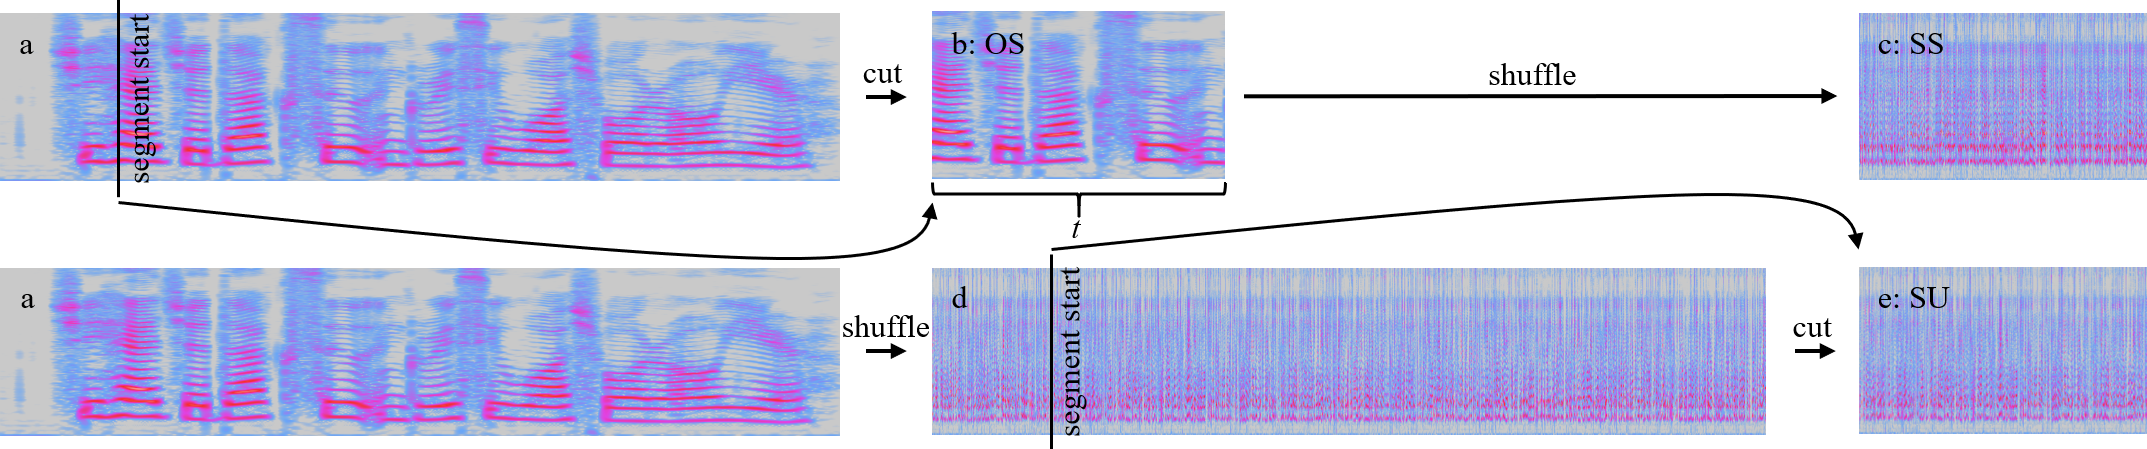
\includegraphics[width=1.0\linewidth]{img/segment-drawing.png}
%     \caption{Erzeugung und Vertauschung von Segmenten (adaptiert von \cite{neururer2023deep}).}
%     \label{shuffle_sst_exploitation}
% \end{figure}

% In der genannten Studie werden verschiedene \gls{dnn}-Modelle für Sprechererkennung (\gls{sv}) und -verifizierung (\gls{sc}) auf unterschiedlichen Trainings- und Auswertungsdatensätzen getestet. Dies umfasst das Training auf den originalen Segmenten (OS) und die Auswertung auf OS, SS und SU sowie das Training auf SS und die Auswertung auf OS, SS und SU und das Training auf SU und die Auswertung auf OS, SS und SU. Die Ergebnisse sind in der folgenden Grafik dargestellt.

% \begin{figure}[h]
%     \centering
%     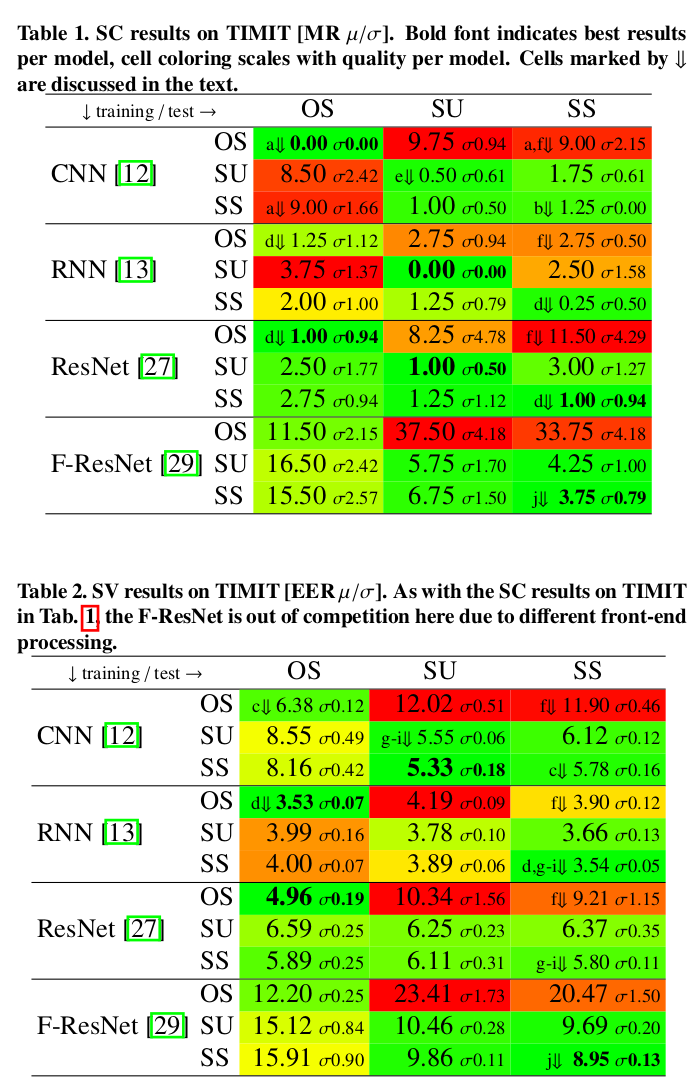
\includegraphics[width=0.54\linewidth]{img/neururer_resultate.png}
%     \caption{Testergebnisse von \gls{sc} und \gls{sv} unter Verwendung von originalen und vertauschten Segmenten (adaptiert von \cite{neururer2023deep}).}
%     \label{sst_exploitation_results}
% \end{figure}


% Insbesondere zeigt sich aus den Ergebnissen, dass das Training und die Auswertung auf vertauschten Daten (SS/SS und SU/SU) State-of-the-Art-Leistungen in \gls{sc} und \gls{sv} liefern, obwohl das Modell keine \gls{sst} nutzt. Diese Ergebnisse werfen erhebliche Zweifel darüber auf, ob \gls{dnn} überhaupt \gls{sst} erlernen oder ob sie sich ausschließlich auf \gls{fba}-Merkmale verlassen \cite{neururer2023deep}.

% Falls die Performance von Training und Evaluation auf den geshuffelten Daten signifikant tiefer als die Performance von Training und Evaluation auf den originalen Daten ist, so kann ausgesagt werden, dass das Model sowohl auf die \gls{fba} als auch \gls{sst} angewiesen ist. Die vorliegende Arbeit untersucht daher die Performance von Transformer Netzwerken in \gls{sv} Tasks und versucht festzustellen, ob Transformer Netzwerke auf \gls{sst} angewiesen sind. 











\chapter{Methods}
\label{chapter:methods}
% 3. Methods [title could be made less generic]
% - [Describe and argue for own methodology/approach: how does your approach work, why did you choose it? The latter could also be discussed in ch. 2]



\section{Overview}

Our experimental framework utilizes the \gls{ssast} model developed by \cite{gong2022ssast}. The architecture of this model is depicted in Figure \ref{fig:ssast_architecture}.

\begin{figure}[h]
    \centering
    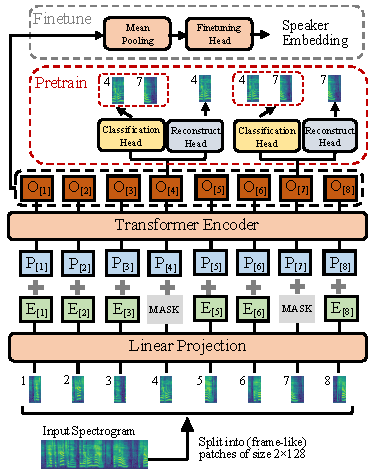
\includegraphics[width=0.6\linewidth]{img/ssast_architecture_frame.pdf}
    \caption{Architecture of the (frame-based) SSAST (adapted from \cite{gong2022ssast}).}
    \label{fig:ssast_architecture}
\end{figure}

To assess the impact of temporal structure in audio spectrograms for \gls{sv} tasks, we compare the performance of models trained on unaltered spectrograms with those trained on temporally shuffled spectrograms.

\section{Data}
\label{methods_datasets}

\subsection{Conversion to Mel Spectrogram}
\label{sec:mel_spectrogram_conversion}

Given a discrete audio waveform ${s} \in \mathbb{R}^l$ sampled at a sampling frequency $f_s$, where ${s}[n]$ denotes the $n$-th sample in the audio signal and $l$ is the number of samples in the audio signal, the Mel spectrogram can be computed\footnote{See \href{https://pytorch.org/audio/main/\_modules/torchaudio/compliance/kaldi.html\#fbank}{https://pytorch.org/audio/main/\_modules/torchaudio/compliance/kaldi.html\#fbank} for more details.} as described in the following paragraphs \cite{yang2021torchaudio, hwang2023torchaudio}. Figure \ref{fig:main_steps_signal_into_melspectrogram} illustrates the main steps of the conversion on a high level.

\begin{figure}[h]

    \centering
    
    \begin{tikzpicture}[
            font=\footnotesize, 
            %thick, 
            node distance=0.45cm, 
            auto 
        ]
        
        % Define styles
        \tikzstyle{block} = [rectangle, draw, text width=4.6em, text centered, minimum height=3.5em]
        \tikzstyle{line} = [draw, -Latex]

    
         % Nodes
         
        \node (acoustic) {
\includegraphics[scale=0.9, clip, viewport=0 0 0.166\imagewidth{} 0.93\imageheight{}]{img/waveform.pdf}};
        
        \node[block, right=0.7cm of acoustic] (windowing) {
            \begin{tikzpicture}[yscale=1, xscale=0.8]
                \draw[smooth, domain=-1:1, samples=20, variable=\x] plot ({\x}, {0.5*(cos(deg(0.5*pi*\x)))^2});
            \end{tikzpicture}
        };

        \node[block, right=0.8cm of windowing] (fourier) {$t \xrightarrow{\text{\Large$\mathscr{F}$}} f$};
        
        % \node[block, right=0.8cm of fourier] (melbank) {};
        % % mel fbanks
        % \setlength{\melwidth}{4.2em} 
        % \setlength{\melheight}{1em}
        % \draw ([shift={(0.0\melwidth, 0.0\melheight)}]melbank.south west) -- ([shift={(0.064\melwidth, 1.0\melheight)}]melbank.south west) -- ([shift={(0.145\melwidth, 0.0\melheight)}]melbank.south west);
        \node[block, right=0.8cm of fourier] (melbank) {
            \begin{tikzpicture}
                \setlength{\melwidth}{5.4em} 
                \setlength{\melheight}{2.3em}
                \draw[red!60!black] (0.0\melwidth, 0.0\melheight) -- (0.064\melwidth, 1.0\melheight) -- (0.145\melwidth, 0.0\melheight);
                \draw[red!80!black] (0.064\melwidth, 0.0\melheight) -- (0.145\melwidth, 1.0\melheight) -- (0.246\melwidth, 0.0\melheight);
                \draw[red] (0.145\melwidth, 0.0\melheight) -- (0.246\melwidth, 1.0\melheight) -- (0.375\melwidth, 0.0\melheight);
                \draw[orange!20!red] (0.246\melwidth, 0.0\melheight) -- (0.375\melwidth, 1.0\melheight) -- (0.537\melwidth, 0.0\melheight);
                \draw[orange!60!red] (0.375\melwidth, 0.0\melheight) -- (0.537\melwidth, 1.0\melheight) -- (0.741\melwidth, 0.0\melheight);
                \draw[orange] (0.537\melwidth, 0.0\melheight) -- (0.741\melwidth, 1.0\melheight) -- (1.0\melwidth, 0.0\melheight);
            \end{tikzpicture}
        };

        \node[right=0.7cm of melbank] (melspec) {\includegraphics[scale=0.8, clip, viewport=0 0 0.168\imagewidth{} 1.0\imageheight{}]{img/spectrogram.pdf}};

        % Arrows
        \draw[line] (acoustic) -- ($(windowing.west) - (0.3em, 0)$);
        \draw[line] ($(windowing.east) + (0.3em, 0)$) -- ($(fourier.west) - (0.3em, 0)$);
        \draw[line] ($(fourier.east) + (0.3em, 0)$) -- ($(melbank.west) - (0.3em, 0)$);
        \draw[line] ($(melbank.east) + (0.3em, 0)$) -- (melspec);

                % Labels
        \coordinate (LabelBase) at ([yshift=0.4em]acoustic.north);
        \node[anchor=base] at (LabelBase -| acoustic) {Raw Waveform};
        \node[anchor=base] at (LabelBase -| windowing) {Windowing};
        \node[anchor=base] at (LabelBase -| fourier) {Fourier Transform};
        \node[anchor=base] at (LabelBase -| melbank) {Mel Filters};
        \node[anchor=base] at (LabelBase -| melspec) {Mel Spectrogram};
        
    \end{tikzpicture}

    \caption{Main steps for converting an acoustic signal into a Mel spectrogram.}
    \label{fig:main_steps_signal_into_melspectrogram}
\end{figure}


\subsubsection{Windowing and Frame Striding}
The signal \({s}\) is divided into overlapping frames using a stride of \(S\) and a window length of \(W\). This results in \(L\) frames where 
\begin{equation}
\label{eq:spectrogram_L}   
L = \left\lfloor \frac{l - W}{S} + 1 \right\rfloor.
\end{equation}
The floor function, denoted by \(\lfloor \cdot \rfloor\), ensures that only complete frames are used. Each frame \({s}_i\), where \(i \in \{0, 1, \ldots, L-1\}\), is centered as follows:
\begin{equation}
\label{eq:timedomain_frames}
{s}_i = ({s}[h : h+W-1] - \mu_{{s}_i}), \quad \text{for } h = i \cdot S,
\end{equation}
where \(\mu_{{s}_i}\) is the mean of the frame.

\subsubsection{Pre-emphasis Filtering}
After centering, a pre-emphasis filter is applied to each frame to accentuate higher frequencies:
\begin{equation}
\label{eq:preemphasis}
{s}_i'[n] = {s}_i[n] - \alpha \cdot {s}_i[n-1]
\end{equation}
where \(\alpha = 0.97\) is the pre-emphasis coefficient.

\subsubsection{Window Function}
To minimize spectral leakage, each frame \({s}_i'\) is then multiplied element-wise with a window:
\begin{equation}
{s}_i'' = {s}_i' \odot {w}
\end{equation}
where \({w}\) is obtained using a windowing function (e.g. Hanning).


\subsubsection{Fourier Transform and Power Spectrum}
Each frame is zero-padded to the nearest power of two, \(W_{\text{pad}}\), and transformed into the frequency domain using the \gls{fft} \cite{Cooley1965}. The power spectrum \({P}_i\) of each frame is computed as:
\begin{equation}
\label{eq:power_spectrum} 
{P}_i = \left| \mathscr{F}({s}_i'') \right|^2 \in \mathbb{R}^{\frac{W_{\text{pad}}}{2}+1}
\end{equation}
where \(\mathscr{F}\) denotes the \gls{fft} for a real-valued input signal. These power spectra are then concatenated as columns to create ${P}$, a matrix of size $\left( \frac{W_{\text{pad}}}{2}+1 \right) \times L$.

\subsubsection{Mel Filter Banks}
The Mel scale filter banks are applied to the power spectrum to extract frequency bands that correspond to human auditory perception. This is achieved by mapping frequencies onto the Mel scale, which is calculated using the following conversions:
\begin{align}
m(f) &= 1127 \log_e \left(1 + \frac{f}{700}\right) \label{eq:mel-scale-to-mel} \\
f(m) &= 700 \left(e^{m / 1127} - 1\right) \label{eq:mel-scale-to-hz}
\end{align}
The filter banks ${H}$, a matrix of size $M \times \left(\frac{W_{\text{pad}}}{2}+1\right)$, transform the power spectra to the Mel scale. The calculation of ${H}_{ij}$ in the Mel filter banks involves constructing triangular filters between specific points on the frequency scale. For each filter $i$ the coefficients are computed as follows:
\begin{equation}
{H}_{ij} = 
\begin{cases} 
\frac{m(f_j) - m_{\text{left}}}{m_{\text{center}} - m_{\text{left}}}, & \text{if } m_{\text{left}} \leq m(f_j) < m_{\text{center}}, \\
\frac{m_{\text{right}} - m(f_j)}{m_{\text{right}} - m_{\text{center}}}, & \text{if } m_{\text{center}} \leq m(f_j) < m_{\text{right}}, \\
0, & \text{otherwise}.
\end{cases}
\end{equation}
where $f_j$ is the center frequency of the $j$-th bin in the Fourier transformed frame, $m_{\text{left}}$, $m_{\text{center}}$, and $m_{\text{right}}$ are the mel frequencies corresponding to the left, center, and right edges of the $i$-th triangular filter, respectively.

Figure \ref{fig:mel-filter-matrix} shows the structure of the matrix ${H}$ in the case of $f_s=16\text{kHz}$, $M=128$ and $W_{\text{pad}}=512$.
\begin{figure}[h]
    \centering
    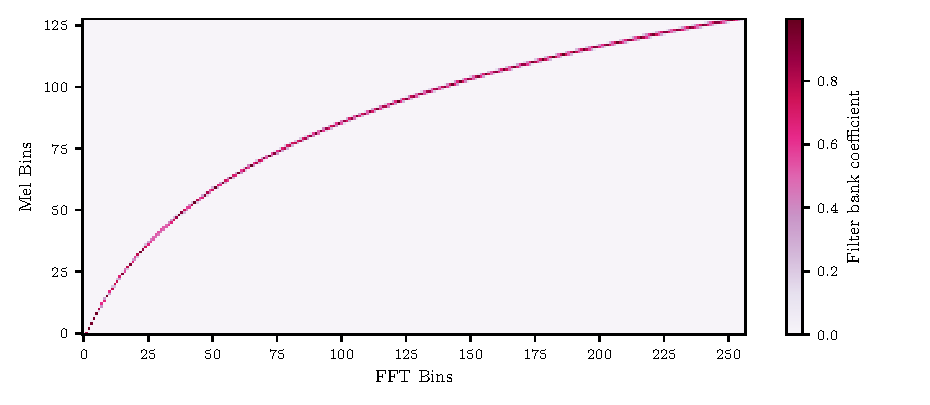
\includegraphics[width=1.0\linewidth]{img/plots/mel_filter_bank_matrix.pdf}
    \caption{Mel filter bank matrix ${H}$ in the case of $f_s=16\text{kHz}$, $M=128$ and $W_{\text{pad}}=512$.}
    \label{fig:mel-filter-matrix}
\end{figure}

\subsubsection{Application of the Filter Banks}
Finally, the obtained Filterbanks ${H}$ are applied to ${P}$ and the logarithm is computed:
\begin{equation}
{X} = \log_e({H} {P} + \epsilon) \in \mathbb{R}^{M \times L}
\end{equation}
where $\epsilon$ is a small constant to avoid logarithm of zero.

This results in ${X}$, the Mel spectrogram, where $M$ is the number of Mel bins and $L$ is the number of frames. Each frame of the Mel spectrogram is denoted as ${X}[i]$, for $i = 0, 1, \ldots, L-1$.

\subsection{Datasets}

For the pretraining task, we use AudioSet-2M \cite{gemmeke2017audio} and Librispeech \cite{panayotov2015librispeech}, enabling comparison with the results reported in \cite{gong2022ssast} and thus facilitating validation of our experimental setup and codebase. Combined, these two datasets consist of 5,734 hours of audio. 

For fine-tuning on \gls{sv}, in addition to the Librispeech dataset the VoxCeleb dataset \cite{nagrani2017voxceleb} is used. It comprises a diverse collection of speakers recorded in various settings, providing a rich landscape for assessing \gls{sv} efficacy. Combined, these two datasets consist of 3,368 hours of audio from 9,593 distinct speakers.

All audio files are converted to $f_s=16$kHz mono channel audio signals of 10 seconds, i.e. one-dimensional arrays of $l=160{,}000$ values. If the original audio file is longer than that, it is split into pieces. For audio files shorter than 10s, they are combined with other files.

As a preprocessing step, audio files are converted into mel spectrograms, using the procedure outlined in \ref{sec:mel_spectrogram_conversion}. Each spectrogram $X$ consists of $L$ frames with $M$ mel bins. A single frame covers a duration of 25 milliseconds ($\Rightarrow W=16\text{kHz}\cdot25\text{ms}=400$), and consecutive frames are shifted by 10 milliseconds ($\Rightarrow S=16\text{kHz}\cdot10\text{ms}=160$) relative to each other. The number of frames in a 10-second audio clip can be calculated using Equation \ref{eq:spectrogram_L}:
$$
L = \left\lfloor \frac{l - W}{S} + 1 \right\rfloor = \left\lfloor \frac{160000 - 400}{160} + 1 \right\rfloor = 998
$$
This calculates the total number of 25ms frames that can fit into 10 seconds, taking into account that each subsequent frame starts 10ms after the previous one. The number of Mel bins $M$ is set to 128 and a Hanning window is used. Consequently, the preprocessed data samples are all of size $998 \times 128$:
\[
    X =
    \begin{bmatrix}
    \vert & \vert & \vert & \vert & \vert &       & \vert  \\
    X[0]  & X[1]  & X[2]  & X[3]  & X[4]  &\cdots & X[997] \\
    \vert & \vert & \vert & \vert & \vert &       & \vert
    \end{bmatrix}
    \in \mathbb{R}^{128 \times 998}
\]


\section{Pretraining}
\label{methods_pretraining}

In this section, we describe the self-supervised pretraining algorithm developed by \cite{gong2022ssast}. As opposed to frameworks that either used a discriminative (e.g., wav2vec \cite{schneider2019wav2vec}) or a generative (e.g., APC \cite{chung2020generative}) loss function, the \gls{ssast} architecure employs a joint discriminative and generative objective for pretraining, which is summarized in Algorithm~\ref{alg:pretrain}.

\begin{algorithm}[h]
\caption{Joint Discriminative and Generative Masked Spectrogram Patch Modeling}
\label{alg:pretrain}
\begin{algorithmic}[1]
\Require{Unlabeled Audio Dataset $\mathcal{D}$, SSAST Model $\mathcal{M}$, Number of Masked Patches $N$}
\For{every epoch}
    \For{$X \in \mathcal{D}$}
        \State split $X$ into $T$ patches $x=\{x_0, x_1, ..., x_{T-1}\}$
        \State $E=\mathcal{M}_{\texttt{patch\_embedding}}(x)$ 
        \State $I=\text{RandomSample}(\{0, 1, \dots, T-1\}, N)$ \Comment{Select $N$ unique indices}
        \State $E_I$ = $E_{\texttt{mask}}$ \Comment{Mask the Patch Embeddings}
        \State $O=\mathcal{M}_{\texttt{Transformer}}(E+P)$
        \State $\mathcal{L}_d=0,\mathcal{L}_g=0$
        \For{$i\in I$}
            \State $r_i=\mathcal{M}_{\texttt{reconstruction\_head}}(O_i)$
            \State $c_i=\mathcal{M}_{\texttt{classification\_head}}(O_i)$
            \State $\mathcal{L} \mathrel{+}= \mathcal{L}_d(x_i,c_i,x_I) + \lambda\mathcal{L}_g(x_i,r_i)$
        \EndFor
        \State$\mathcal{L} = \mathcal{L}\mathbin{/}N$
        \State update $\mathcal{M}$ to minimize $\mathcal{L}$ 
    \EndFor
\EndFor 
\Return $\mathcal{M}$
\end{algorithmic}
\end{algorithm}

As mentioned above, the spectrograms $X$ are of size $998\times128$. They are then split into $T=L/2=499$ patches $x=\{x_0, x_1, ..., x_{498}\}$ of size $2 \times 128$ (2 frames in the time dimension with 128 mel frequency bins). These \textit{frame-like} patches $x$ henceforth serve as the basic processing unit of the model, similar to the subword tokens in an \gls{llm}:
\[
\underbrace{\begin{array}{cc}
\vert & \vert \\
X[0] & X[1] \\
\vert & \vert
\end{array}}_{x_0}
\underbrace{\begin{array}{cc}
\vert & \vert \\
X[2] & X[3] \\
\vert & \vert
\end{array}}_{x_1}
\cdots
\underbrace{\begin{array}{cc}
\vert & \vert \\
X[996] & X[997] \\
\vert & \vert
\end{array}}_{x_{498}}
\]

Each patch $x_i$ is converted to a corresponding 768-dimensional patch embedding $E_i$ using a linear projection layer, which is called \texttt{patch\_embedding}-layer. Then a set of indices $I$ is generated by randomly sampling $N$ unique numbers from $\{0, 1, ..., 498\}$. For each patch $x_i$ with an index $i \in I$, its patch embedding is replaced with a learnable mask embedding $E_{\texttt{mask}}$. Then, positional embeddings $P$ (also learnable) are added to the patch embeddings $E$ and the result is input to the (encoder-only) Transformer. Thus, the Transformer output $O$ ($499\times768$) is obtained. For each of the masked patches $x_i$, its corresponding $O_i$ is input to a classification head and a reconstruction head to get an output $c_i$ and $r_i$, respectively. 

The Transformer has an embedding dimension of 768, 12 layers, and 12 heads. Both the classification and reconstruction heads are two-layer \glspl{mlp} that map $O_i$ (768) to the same dimension as the (flattened) input patch $x_i$ (256). $r_i$ is expected to be close to $x_i$, and the model should learn to match correct ($x_i, c_i$) pairs. Therefore, the \gls{mse} loss $\mathcal{L}_g$ is used for the generative objective and the \gls{infonce} loss~\cite{oord2018representation} $\mathcal{L}_d$ for the discriminative objective:
\begin{equation}
\label{eq:MSE}
\mathcal{L}_g=\frac{1}{N}\sum_{i \in I} \text{mean}\left((r_i-x_i)^2\right)
\end{equation}
\begin{equation}
\label{eq:InfoNCE}
\mathcal{L}_d=\frac{-1}{N}\sum_{i \in I}\log_e\left(\frac{\exp(c_i * x_i)}{\sum_{j \in I}\exp(c_i * x_j)}\right)
\end{equation}
where $N$ is the number of masked patches and $*$ denotes the dot product. $\mathcal{L}_d$ and $\mathcal{L}_g$ are then added with a weight $\lambda$:
\begin{equation}
\label{eq:pretraining-loss}
\mathcal{L}=\mathcal{L}_d + \lambda\mathcal{L}_g
\end{equation}
Akin to \cite{gong2022ssast}, we set $\lambda=10$. Finally, the parameters are updated to minimize $\mathcal{L}$ using the \gls{adam} optimizer \cite{kingma2015adam}. 

The authors of \cite{gong2022ssast} found out that frame-based \gls{ssast} results in superior performance compared to patch-based \gls{ssast} for speech-related downstream tasks. Furthermore, they also found that masking $N=400$ of the $T=512$ frame-like patches surpasses masking $N=250$ patches. Consequently, we adopt this masking approach during pretraining, masking $N=390$ of the $T=499$ frame-like $2 \times 128$ patches for the pretraining, to obtain a similar ratio of number of masked patches $N$ / total number of patches $T$. During evaluation, we accidentily used $N=400$, making the task a bit harder during evaluation\footnote{Our code built on \cite{gong2022ssast}, and they always used $N=400$ for evaluation, independent of the number of masked patches used for training.}.

\glsunset{mo}%
\glsunset{ms}%
Two distinct pretraining instances are initiated using the \gls{ssast} architecture:
\vspace{-\parskip}
\begin{itemize}[topsep=0.5\parskip, itemsep=0.0\parskip, parsep=0.5\parskip]
    \item Pretraining on original spectrograms for 10 epochs (\gls{mo}).
    \item Pretraining on spectrograms with their frames shuffled randomly in time, disrupting the temporal structure (\gls{ms}). Since the losses quickly stabilize at the expected values (Algorithm \ref{alg:mse_shuffled} and Equation \ref{eq:expected_infonce}), 5 epochs are enough for this configuration.
\end{itemize}

This dual approach is designed to yield insights into the influence of the temporal spectrogram arrangement during pretraining on the model's learning process. While shuffling the frames eliminates the model's ability to leverage temporal features, the model can still make some predictions, such as assigning an equal probability to all masked patches in the classification task and predicting the average of the unmasked patches in the reconstruct head. 

We set the batch size to 48, which is twice as much as the original \gls{ssast}. We use an initial learning rate of $10^{-4}$, and cut it into half if the patch prediction accuracy on the validation set stops improving for 8k iterations. We pretrained the \gls{ssast} on 3 NVIDIA A100 GPUs, which took about 4.4 days in the case of the model trained on original spectrograms (\gls{mo}) and 2.2 days in the case of the model trained on shuffled spectrograms (\gls{ms}). 



\section{Finetuning}
\label{sec:met:finetuning}

\glsunset{moo}%
\glsunset{mos}%
\glsunset{mso}%
\glsunset{mss}%
Both models, \gls{mo} and \gls{ms}, having undergone pretraining as described in \ref{methods_pretraining}, are then finetuned for \gls{sv} on the VoxCeleb 1/2 and Librispeech dataset. The dataset for finetuning consists of 3368 hours of speaker utterances from 9593 different speakers. The fine-tuning protocol, including mean-pooling on the outputs of the transformer encoder followed by a linear layer to derive speaker embeddings, is executed as delineated in \cite{gong2022ssast}. Corresponding to the pretraining phase, fine-tuning is done on both the original ($\Rightarrow \mathcal{M}_\text{$\cdot$/o}$) and the shuffled ($\Rightarrow \mathcal{M}_\text{$\cdot$/s}$) spectrograms for each of the two pretraining conditions, which yields four distinct models, referred to as \gls{moo}, \gls{mos}, \gls{mso} and \gls{mss}.

To finetune the two pretrained models on the downstream task of \gls{sv} the main idea is to project the transformer embeddings into a new vector space where it is possible to differentiate between two speakers using a vector similarity metric \cite{chung2020ContrastiveLoss, chung2018voxceleb2}. The paper \cite{chung2018voxceleb2} showed a proof of concept for this strategy. It used the same dataset (VoxCeleb) for training and as the speaker embedding dimension 512 was chosen. 

This thesis investigates three different approaches to finetune the \gls{ssast} model; experiment 1 (\ref{methods_finetune_firstAttempt}), experiment 2 (\ref{methods_finetune_secondAttempt}) and experiment 3 (\ref{methods_finetune_thirdAttempt}).

\subsection{Experiment 1}
\label{methods_finetune_firstAttempt}
For the first experiment the same \gls{mlp} structure is used as suggested in the finetuning part in \cite{gong2022ssast}. It consists of a LayerNormalization and a fully connected layer with an input dimension of 768 and an output dimension of 527, which is very close to the approach described in \cite{chung2018voxceleb2}. As described above, both pretrained models are finetuned once on original spectrograms and once on shuffled spectograms. The performance of these four different models, \gls{moo}, \gls{mos}, \gls{mso} and \gls{mss}, is evaluated on original spectrograms and shuffled spectrograms using 100 different speakers from the dataset used for finetuning.

\subsection{Experiment 2}
\label{methods_finetune_secondAttempt}
In the second experiment, an \gls{mlp} is used with an output dimension of 256 and the same architecture as deployed in the classification head during the pretraining stage. The idea behind it is that the pretraining loss forces the classification head to create correct matches of masked patches and the corresponding embeddings. Therefore, this architecture should also have the potential to accurately generate inter- and intra-speaker embeddings. For performance evaluation 100 different speakers from the finetuning dataset have been used.

\subsection{Experiment 3}
\label{methods_finetune_thirdAttempt}
During evaluation and after consultations with our supervisor, Prof. Dr. Thilo Stadelmann, we have reasons to believe that the training time in Experiment~1 (Section \ref{methods_finetune_firstAttempt}) was not sufficient. Therefore a third experiment has been set up. It uses the same head as described in Experiment~1 (Section \ref{methods_finetune_firstAttempt}) because, as discussed in \ref{results_finetuning}, this head yields the most promising performance. This experiment has been run for 14 Epochs on the same dataset as described in \ref{sec:met:finetuning}. Unfortunatly, it was not possible for us to let the experiment run for more epochs due to time limitations. For performance evaluation 100 different speakers from the finetuning dataset have been used.

\subsection{Loss}
\label{methods_contrastive_loss}

For contrastive learning there are different loss functions that have been widely used in state-of-the-art \gls{sr} \cite{chung2020ContrastiveLoss, bjorn2019cosineloss}. The loss functions relevant for this thesis are discussed in the following subsections. 

The first approach was to use the triplet loss. This decision has been made because of the wide use of the triplet loss function in this domain. The downside of the triplet loss was that the implementation could not be made very efficient as we wanted it to be, because our code used a for-loop to iterate over the different output embeddings to calculate the loss. When using the cosine embedding loss, we were able to vectorize the loss calculation, which lead to faster training. The required time per sample for the triplet loss was 0.017 seconds on average. With the cosine embedding loss the time per sample decreased by almost 20\% to 0.014 seconds. 

To finalize our decision, we compared the performance of the two approaches by finetuning with both setup for one day. We have achieved similar results in terms of performance and therefore the more efficient implementation has been used. 


\subsubsection{Triplet Loss}
The triplet loss \cite{Schroff2015FaceNetAU} was our first approach. It is computed using the following equation:
% \begin{equation}
% \label{eq:triplet}
% \mathcal{L}(A, P, N)=\max \left(\|f(A)-f(P)\|_p-\|f(A)-f(N)\|_p+\alpha, 0\right)
% \end{equation}
\begin{equation}
\label{eq:triplet}
\mathcal{L}=\max \left(\|\mathcal{M}(X_A)-\mathcal{M}(X_P)\|_p-\|\mathcal{M}(X_A)-\mathcal{M}(X_N)\|_p+\alpha, 0\right)
\end{equation}
We set $p = 2$ and $\alpha = 1$, which is also the default for PyTorch \cite{paszke2019pytorch, PyTorchTripletMarginLoss}. In Equation \ref{eq:triplet}, $\mathcal{M}(X_A)$ denotes the output of the model (i.e. the speaker embedding) for the audio sample of an \textit{anchor} speaker, $\mathcal{M}(X_P)$ represents the embedding of an audio sample of the same speaker (a \textit{positive} sample) and $\mathcal{M}(X_N)$ is the embedding of a different speaker (a \textit{negative} sample). During the training process $\mathcal{M}(X_A)$ and $\mathcal{M}(X_P)$ are pulled closer to each other, while $\mathcal{M}(X_A)$ and $\mathcal{M}(X_N)$ are pulled apart, as illustrated in Figure \ref{fig:triplet_loss}.

\begin{figure}[h]
  \centering

  \begin{tikzpicture}[scale=1, every node/.style={font=\scriptsize}]
    % Define styles
    \tikzset{
      main node/.style={circle, draw, minimum size=0.4cm, inner sep=0},
      label node/.style={circle, minimum size=0.3cm}
    }

    % Define offset for right side nodes
    \newcommand{\offset}{10}


    % Left side

    % Place text node outside the circle
    \node[main node, fill=blue!30] (a) at (0,0) {};
    \node[above left=-0.15cm of a] {$\mathcal{M}(X_A)$};

    % Circles with margin label for left side
    \draw[thick] (a) circle (2.6cm);
    \draw[thick] (a) circle (1.5cm);
    \draw[thick, <->] (-2.6,0) -- node[above, fill=white] {\small$\alpha$} (-1.5,0);

    % Use polar coordinates for positioning nodes
    \node[main node, fill=red!30] (n) at (-45:1.5) {};
    \node[below=0.1cm of n.east, anchor=north] {$\mathcal{M}(X_N)$};
    \node[main node, fill=green!30] (p) at (30:3) {};
    \node[above=0.1cm of p.east] {$\mathcal{M}(X_P)$};
    \draw[thick, -Stealth] (a) -- (n);
    \draw[thick, -Stealth] (a) -- (p);


    % Right side

    % Place text node outside the circle
    \node[main node, fill=blue!30] (a2) at (\offset,0) {};
    \node[above left=-0.15cm of a2] {$\mathcal{M}(X_A)$};

    % Circles with margin label for right side
    \draw[thick] (a2) circle (2.6cm);
    \draw[thick] (a2) circle (1.5cm);
    \draw[thick, <->] (\offset - 2.6,0) -- node[above, fill=white] {\small$\alpha$} (\offset - 1.5,0);

    % Use polar coordinates for positioning nodes with offset
    \node[main node, fill=red!30] (n2) at ([shift={(\offset,0)}]-30:2.7) {};
    \node[below right=-0.2cm of n2] {$\mathcal{M}(X_N)$};
    \node[main node, fill=green!30] (p2) at ([shift={(\offset,0)}]45:1.4){};
    \node[above right=-0.2cm of p2.north east, anchor=south west] {$\mathcal{M}(X_P)$};
    \draw[thick, -Stealth] (a2) -- (n2);
    \draw[thick, -Stealth] (a2) -- (p2);


    % Training Arrow

    \path (a) -- (a2) node[midway, single arrow, draw=black, minimum width=20mm, minimum height=30mm, inner sep=0mm, single arrow head extend=3mm] {\normalsize Training};

  \end{tikzpicture}

  \caption{Visualization of the Triplet loss (adapted from \cite{matties2020vector}).}
  \label{fig:triplet_loss}
\end{figure}


\subsubsection{Cosine embedding loss}

The cosine embedding loss was the final loss function used for further evaluation. For two speakers with identity labels $a$ and $b$, it is computed using the following equation:
\begin{equation}
 \mathcal{L}= \begin{cases}1 - \operatorname{sim} \left(\mathcal{M}(X_a), \mathcal{M}(X_b)\right), & \text { if } a = b \\ \max \left(0, \operatorname{sim} \left(\mathcal{M}(X_a), \mathcal{M}(X_b)\right)-\alpha\right), & \text { if } a \neq b \end{cases},
\end{equation}
where $\mathcal{M}(X)$ is the output of the model for a Mel spectrogram $X$ and $\operatorname{sim}(\cdot, \cdot)$ denotes the cosine similarity of two vectors:
\begin{equation}
\operatorname{sim}(u, v) := \cos(\theta) = \frac{u * v}{\|u\| \|v\|}=\frac{\sum_{i=1}^n u_i v_i}{\sqrt{\sum_{i=1}^n u_i^2} \sqrt{\sum_{i=1}^n v_i^2}}.
\end{equation}
We set $\alpha=0$, which is also the default in Pytorch.




\subsection{Testing}

Each finetuned model is scrutinized under the same two testing conditions; on shuffled as well as on orinial spectrograms. This evaluation strategy is pivotal to discern whether models leverage temporal features. For performance evaluation, \gls{eer} and cosine similarity are calculated.

\subsubsection{\gls{eer} - Equal Error Rate}

\begin{figure}[htbp] % 'htbp' option is for placement of the figure
    \centering % This centers the figure in the column
        \begin{tikzpicture}
            
            % Improved labels for axes
            \draw[thick,->] (-0.5,0) -- (7.5,0) node[midway, below] {Threshold}; % Label x-axis, shifted downward for clarity
            \draw[thick,->] (0,-0.5) -- (0,4.5) node[midway, above, rotate=90] {Error Rate (\%)}; % Rotated y-axis label, shifted right for clarity

            % Hyperbola
            \draw[domain=0.5:7,variable=\x,smooth,thick] plot ({\x},{2/(\x/1.0)});
            \draw[domain=0.5:7,variable=\x,smooth,thick] plot ({\x},{2/(-((\x/1.0)-7.5))});
        
            % Labels
            \node at (7.5-1.2,3.5) [above] {FRR};
            \node at (1.2,3.5) [above] {FAR};
            
            % Make EER point and label red
            \node at (3.75,0.533) [circle,fill,inner sep=2pt, red]{}; % EER point in red
            \node at (3.75,0.65) [above, red] {EER}; % EER label in red
            
        \end{tikzpicture}
    \caption{Illustration of FAR and FRR curves with EER point.} % Caption for the figure
    \label{fig:eer_curve} % Label for referencing the figure
\end{figure}

The \gls{eer} is a popular benchmark in \gls{sv} for comparing model performance. It is well suited for the performance evaluation of binary classification models. It provides a single value that summarizes the system's performance by balancing two types of errors: false acceptances and false rejections. The \gls{eer} is defined as the point at which the \gls{far} and \gls{frr} are equal, as illustrated in Figure \ref{fig:eer_curve}.

\pagebreak [2]
Using the \gls{eer} as a performance metric makes it possible to conduct the \textsc{Neururer} examination \cite{neururer2023deep} as described in \ref{foundation_sst} and answer the main research question of this thesis.

\subsubsection{Cosine similarity}
In data analysis, cosine similarity is a measure of similarity between two non-zero vectors defined in an inner product space. Cosine similarity is the cosine of the angle between the vectors; that is, it is the dot product of the vectors divided by the product of their lengths. It follows that the cosine similarity does not depend on the magnitude of the vectors, but only on their angle \cite{HAN201239, Singhal2001ModernIR}.

Evaluating this metric can underline the statement beeing made by the \gls{eer} and directly verifies if the finetuned model has learned to differentiate between intra- and inter-speaker embeddings.


\chapter{Results}
\label{chapter:results}
% 4. Experiments & Results
% - [Experimental setup, results, discussion of results incl. their relevancy & limitations; specific organization is very depedenent on the individual situation]
\section{Pretraining}

\subsection{Original Spectrograms}

\begin{figure}[h]
    \centering
    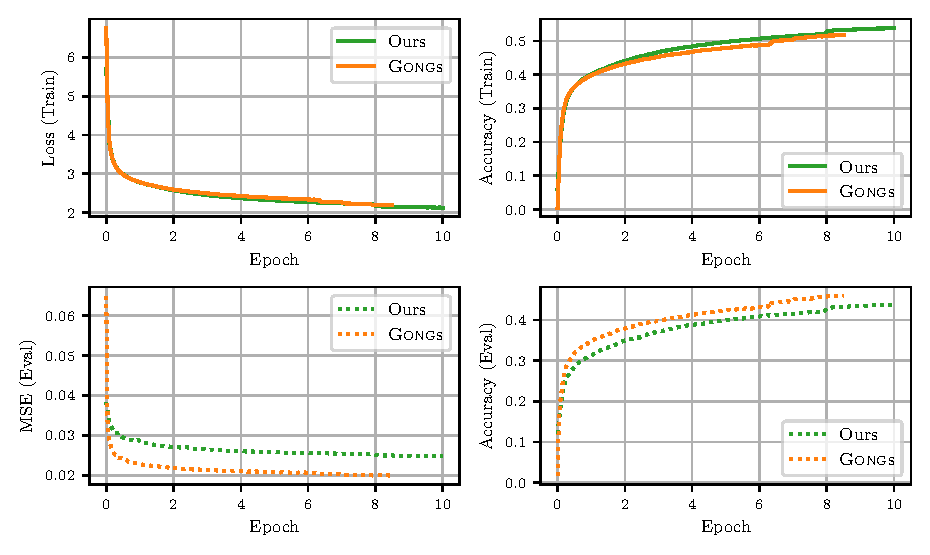
\includegraphics[width=1\linewidth]{img/plots/pretraining_comparison_Gong.pdf}
    \caption{Pretraining result of the model trained on original spectrograms (\gls{mo}).}
    \label{fig:pretrainingResultsOriginalModel}
\end{figure}

Figure \ref{fig:pretrainingResultsOriginalModel} shows the pretraining results of our model trained on original spectrograms (green) compared to the results reported in \cite{gong2022ssast} (orange). The two plots on the top show the performance on the train split, the bottom two plots contain the performance on the test split. The top left plot shows the train loss, calculated using Equation \ref{eq:pretraining-loss}. The bottom left plot shows the \gls{mse} on the test split\footnote{In \cite{gong2022ssast}, they did not keep track of the \gls{infonce} on the evaluation dataset.}. On the right side, we report the accuracy on the train split (top) and the test split (bottom), where accuracy refers to the number of correctly classified patches by the classification head, divided by the total number of masked patches.

As mentioned in \ref{methods_pretraining}, we accidently masked $N=400$ out of $T=499$ patches during evaluation rather than $N=390$, which results in a more challenging task (compared to predicting 400 of 512 patches) and explains the slightly worse performance on the evaluation dataset compared to \cite{gong2022ssast}.

\begin{figure}[h]
    %\begin{adjustwidth}{0cm}{0.0cm}
        \centering
        \begin{tikzpicture}
            \node[anchor=south west,inner sep=0] (image) at (0,0) {
                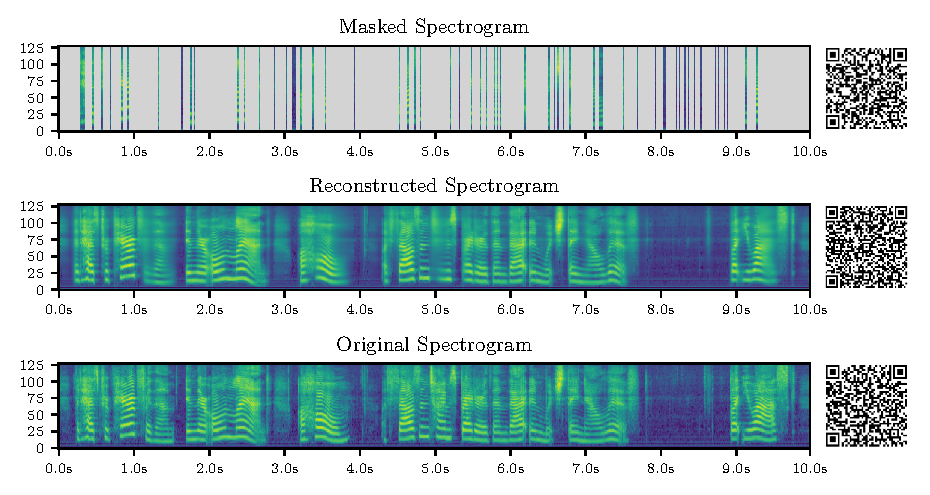
\includegraphics[width=1.0\linewidth]{img/plots/reconstructed_spectrogram_speech_originalModel_with_qr.pdf}
            };
            % Define the scope for the image size
            \begin{scope}[x={(image.south east)},y={(image.north west)}]
                % Define clickable areas
                \node at (0.93,0.18125) {
                    \href{https://github.com/Ironmomo/SpeakerVerificationBA/raw/master/plots_and_audios/audios/original_speech_random_masks_originalModel.wav}{
                        \tikz{\path[fill=none] (0,0) rectangle (0.07,0.165);} % (x, y) ≙ (width, height)
                    }
                };
                \node at (0.93,0.500) {
                    \href{https://github.com/Ironmomo/SpeakerVerificationBA/raw/master/plots_and_audios/audios/reconstructed_speech_random_masks_originalModel.wav}{
                        \tikz{\path[fill=none] (0,0) rectangle (0.07,0.165);}
                    }
                };
                \node at (0.93,0.81875) {
                    \href{https://github.com/Ironmomo/SpeakerVerificationBA/raw/master/plots_and_audios/audios/masked_speech_random_masks_originalModel.wav}{
                        \tikz{\path[fill=none] (0,0) rectangle (0.07,0.165);}
                    }
                };
            \end{scope}
        \end{tikzpicture}
        \caption{Spectrogram with randomly sampled mask indices (top), reconstructed spectrogram from the model trained on original spectrograms (middle), original spectrogram (bottom). Resynthesized audio files from each spectrogram can be downloaded by clicking or scanning the corresponding QR-Code.}
        \label{fig:originalModel_spectrogramReconstruction}
    %\end{adjustwidth}
\end{figure}

Figure \ref{fig:originalModel_spectrogramReconstruction} shows the capabilities of the model pretrained on original spectrograms with an example. In the top part of the image, the masked spectrogram is shown. It is masked at $370$ randomly\footnote{A seed of 15 is used for reproducibility.} sampled indices $I$ in the range $\{0, 1, \dots, 498\}$, i.e., $I=\text{RandomSample}(\{0, 1, \dots, 498\},\linebreak 370)$. This corresponds to 7.4 seconds of masked audio. As seen in the middle spectrogram, the reconstruction is very accurate.





%\newpage

% Difference between \newpage, \clearpage, \pagebreak:
% \newpage ends the current paragraph, fills the current page with white space and starts a new page.
% \clearpage does something more; it also flushes the float queues, producing pages of floats if necessary, then starts a new page.
% \pagebreak is quite different; tells LaTeX to break the current page at the point of the command. With the optional argument, you can convert the \pagebreak command from a demand to a request. The number must be a number from 0 to 4. The higher the number, the more insistent the request is. This command is useful in the last stage of document production: one can force a page break at a convenient spot for improving the typesetting of the next page. Clearly, the text should be in definitive form for this to be effective.


\subsection{Shuffled Spectrograms}

\begin{figure}[hbt!]
    \centering
    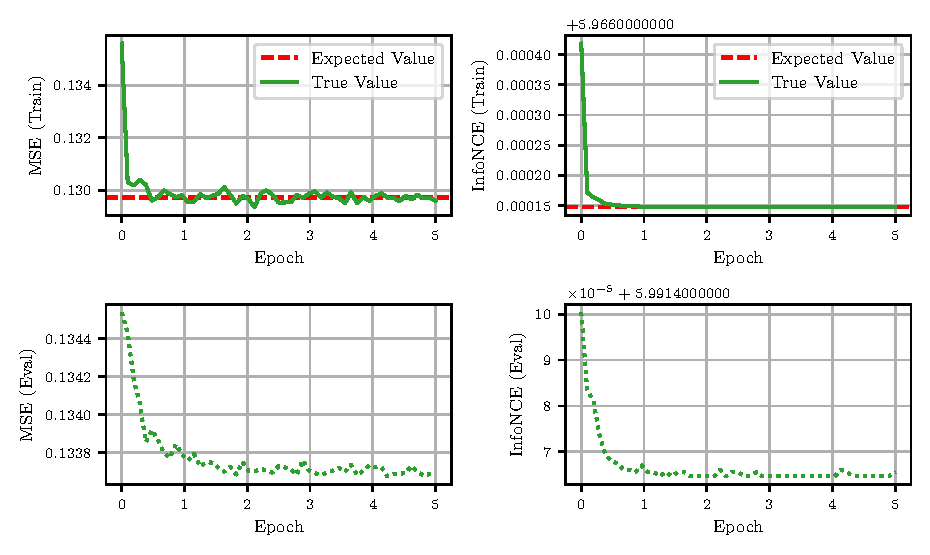
\includegraphics[width=1\linewidth]{img/plots/pretraining_shuffledModel.pdf}
    \caption{Pretraining result of the model trained on shuffled spectrograms (\gls{ms}).}
    \label{fig:pretrainingResultsShuffledModel}
\end{figure}

As seen in Figure \ref{fig:pretrainingResultsShuffledModel}, the loss decreases a bit after the first epoch and then remains more or less at a constant value. The constant value can be calculated for both the \gls{infonce} as well as the \gls{mse} loss. For the train split, this can be done as follows. The procedure for the eval split is analogous.

\begin{algorithm}[hbt!]
\caption{Calculation of Expected \gls{mse} Loss $\mathcal{L}_{g, \text{expected}}$ for the \gls{ms}}
\label{alg:mse_shuffled}
\begin{algorithmic}[1]
\Require{Unlabeled Audio Dataset $\mathcal{D}$, Number of Masked Patches $N$}
\State $\tilde{N}_m = 2N$ \Comment{Number of masked frames}
\State $\tilde{N}_u = L-\tilde{N}_m$ \Comment{Number of unmasked frames}
\State $\texttt{mse\_list} = []$
\For{$X \in \mathcal{D}$}
    \State $I_u=\text{RandomSample}(\{0, 1, \dots, L-1\}, \tilde{N}_u)$ \Comment{Indices of unmasked frames}
    \State $\hat{X} = \frac{1}{\tilde{N}_u} \sum_{i \in I_u} X[i]$ \Comment{Mean vector of unmasked frames}
    \State $I_m = \{0, 1, \ldots, L-1\} \setminus I_u$ \Comment{Indices of masked frames}
    \State $\text{MSE} = \frac{1}{\tilde{N}_m} \sum_{i \in I_m} \text{mean}\left((X[i] - \hat{X})^2\right)$ \Comment{MSE for remaining frames}
    \State Append MSE to $\texttt{mse\_list}$
\EndFor
\State $\mathcal{L}_{g, \text{expected}} = \text{mean}(\texttt{mse\_list})$
\State \textbf{return} $\mathcal{L}_{g, \text{expected}}$
\end{algorithmic}
\end{algorithm}

For the \gls{mse}, the expected loss $\mathcal{L}_{g, \text{expected}}$ can be estimated with Algorithm \ref{alg:mse_shuffled}. The best prediction of a spectrogram with randomly shuffled frames should be to take the average of the unmasked frames as a prediction for the masked ones. To calculate $\mathcal{L}_{g, \text{expected}}$, we can therefore iterate over the dataset, randomly mask $\tilde{N}_m = 2N = 2 \cdot 390 = 780$ frames, calculate the mean in each frequency bin of the remaining $\tilde{N}_u = L-\tilde{N}_m = 998 - 780 = 218$ frames\footnote{The notation $\tilde{N}_m$ and $\tilde{N}_u$ are used to denote the number of masked and unmasked \textit{frames} respectively, to avoid confusion with $N$, which represents the number of masked \textit{patches}.}, and use this as the prediction for the masked frames. Then we calculate the \gls{mse} using Equation \ref{eq:MSE} and take the average over all samples in the dataset, yielding
$$\mathcal{L}_{g, \text{expected}} \approx 0.129726,$$
which seems to be the asymptotic constant{\interfootnotelinepenalty=10000\footnote{To be precise, this value is not exactly the same for each run of Algorithm \ref{alg:mse_shuffled}, since it slightly depends on the (random) selection of the frames used to calculate the average. For a sufficiently large and coherent dataset, this is not a concern.}} the \gls{mse} is approaching.%
%
We can also visualize this property by taking a sample from the dataset, calculating the average of the unmasked frames and plotting a certain number of predicted frames (Figure \ref{fig:average_frame_shuffled_model_predictions}). The predictions are very close to the average of the unmasked frames. This confirms that the model trained on shuffled spectrograms merely learns to calculate the average of the unmasked frames in the spectrogram. The complete masked spectrogram, along with the reconstructed as well as the original spectrogram are shown in Figure \ref{fig:shuffledModel_spectrogramReconstruction}. As can be seen from the middle spectrogram, the reconstruction is very poor, because the model only learned to calculate the average of the unmasked frames in the spectrogram. 

\begin{figure}[hbt!]
    \centering
    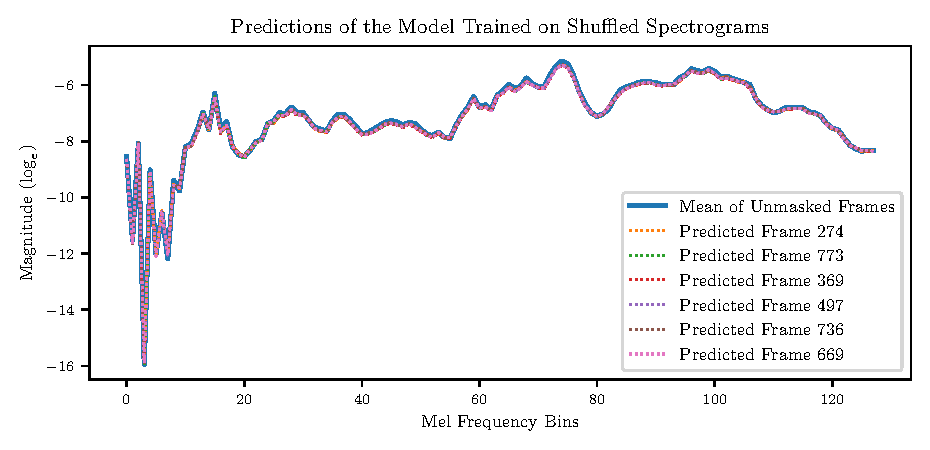
\includegraphics[width=1\linewidth]{img/plots/predictedFrames_shuffled_spectrogram.pdf}
    \caption{Mean of the unmasked frames of the same spectrogram as in Figure~\ref{fig:shuffledModel_spectrogramReconstruction} as well the prediction of the model at six randomly chosen frames from the masked areas.}
    \label{fig:average_frame_shuffled_model_predictions}
\end{figure}

\begin{figure}[hbt!]
    %\begin{adjustwidth}{0cm}{0.0cm}
        \centering
        \begin{tikzpicture}
            \node[anchor=south west,inner sep=0] (image) at (0,0) {
                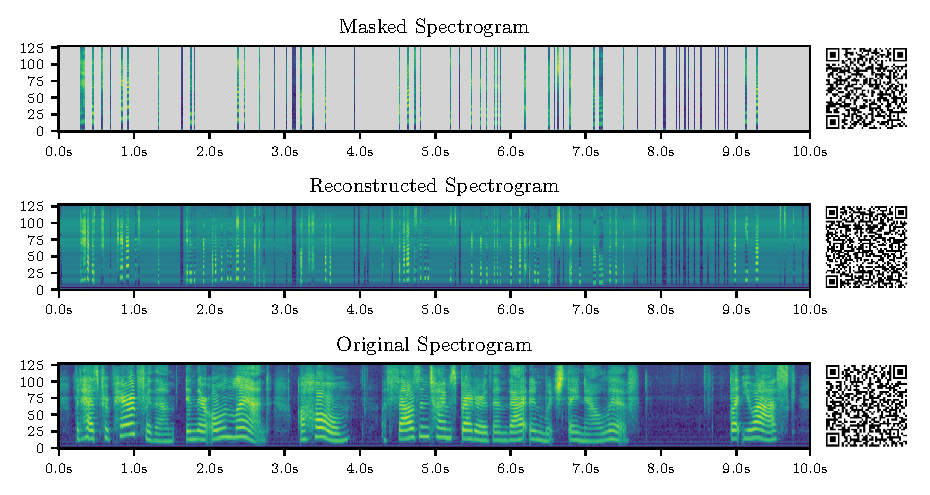
\includegraphics[width=1.0\linewidth]{img/plots/reconstructed_spectrogram_speech_shuffledModel_with_qr.pdf}
            };
            % Define the scope for the image size
            \begin{scope}[x={(image.south east)},y={(image.north west)}]
                % Define clickable areas
                \node at (0.93,0.18125) {
                    \href{https://github.com/Ironmomo/SpeakerVerificationBA/raw/master/plots_and_audios/audios/original_speech_random_masks_shuffledModel.wav}{
                        \tikz{\path[fill=none] (0,0) rectangle (0.07,0.165);} % (x, y) ≙ (width, height)
                    }
                };
                \node at (0.93,0.500) {
                    \href{https://github.com/Ironmomo/SpeakerVerificationBA/raw/master/plots_and_audios/audios/reconstructed_speech_random_masks_shuffledModel.wav}{
                        \tikz{\path[fill=none] (0,0) rectangle (0.07,0.165);}
                    }
                };
                \node at (0.93,0.81875) {
                    \href{https://github.com/Ironmomo/SpeakerVerificationBA/raw/master/plots_and_audios/audios/masked_speech_random_masks_shuffledModel.wav}{
                        \tikz{\path[fill=none] (0,0) rectangle (0.07,0.165);}
                    }
                };
            \end{scope}
        \end{tikzpicture}
        \caption{Spectrogram with randomly sampled mask indices (top), reconstructed spectrogram from the model trained on shuffled spectrograms (middle), original spectrogram (bottom). Resynthesized audio files from each spectrogram can be downloaded by clicking or scanning the corresponding QR-Code.}
        \label{fig:shuffledModel_spectrogramReconstruction}
    %\end{adjustwidth}
\end{figure}

For the \gls{infonce}, each masked frame has an equal probability of being the correct one at any given location. This scenario occurs if 
\begin{equation}
\label{eq:condition_for_equal_prob_infonce}
\frac{\exp(c_i * x_i)}{\sum_{j \in I} \exp(c_i * x_j)} = \frac{1}{N}, \forall i \in I.
\end{equation}

Equation \ref{eq:InfoNCE} can then be simplified as follows:
\begin{equation}
\label{eq:expected_infonce}
\mathcal{L}_{d, \text{expected}} = \frac{-1}{N} \sum_{i \in I} \log_e\left(\frac{1}{N}\right) = \frac{-1}{N} \cdot N \cdot \left(-\log_e(N)\right) = \log_e(N).
\end{equation}

For $N=390$, we obtain
$$\mathcal{L}_{d, \text{expected}} \approx 5.966147,$$
which is exactly the asymptotic value the \gls{infonce} loss approaches, as can be seen in Figure~\ref{fig:pretrainingResultsShuffledModel}. 


\FloatBarrier
\pagebreak [3]
\section{Finetuning}
\label{results_finetuning}

In this section, the results of the finetuning as described in \ref{sec:met:finetuning} are shown and interpreted. This section is structured as follows. First the results of the second finetuning approach (Experiment 2, described in section \ref{methods_finetune_secondAttempt}) using a \gls{mlp} with an output dimension of 256 are discussed. The following sections have been achieved using the first attempt. Exceptions are clearly mentioned. Then the results of the \Gls{eer} are shown and interpreted. Afterwards the results of the cosine similarity are shown and interpreted. The general performance is then evaluated and further interpreted. At the end the results are compared with the \textsc{Neururer} test as described in \ref{foundation_sst}. 

During the last few days before the delivery date of this thesis a 3rd experiment as described in \ref{methods_finetune_thirdAttempt} has been run. The reason for that was because experiment 2 is considered to be a failure. Experiment 3 shows very interesting results leading to another conclusion for this thesis. Due to time concerns the conclusion made from experiment 1 and 2 remains in this thesis. The results of this experiment can be found at the end of this section \ref{results:experiment3}.

\subsection{Experiment 2}

As described in \ref{methods_finetune_secondAttempt}, the second attempt uses a different head to project the (mean pooled) transformer output to speaker embeddings. Due to time limitations only the \gls{ssast} pretrained on the original data, \gls{mo}, has been finetuned, and only on the original data. No further training runs have been done using this head. The model has been trained for 30 epochs. Training it 6x longer than the models trained using approach one (Experiment 1, described in section \ref{methods_finetune_firstAttempt}) should give more insights about the model performance when applying a longer training time. 

\begin{table*}[h]
    \centering
    \caption{Test results of the finetuning using original spectrograms from the Librispeech and Voxceleb 1/2 dataset. \Gls{sr} performance is measured using the \gls{eer}. Bold font indicates best results per model, cell coloring scales with quality per model.}
        \begin{tabular}{>{\centering\arraybackslash}p{1.5cm}| >{\centering\arraybackslash}p{2.5cm} >{\centering\arraybackslash}p{2.5cm}|>{\centering\arraybackslash}p{4cm}  >{\centering\arraybackslash}p{4cm}}
            \hline
            % \multicolumn{2}{c|}{task $\rightarrow$}
            % & \multicolumn{2}{c}{\acrlong{sr}} \\
            \scriptsize{model}
            & \multicolumn{2}{c|}{\scriptsize{pretraining $\downarrow$ / finetuning $\downarrow$ / test $\rightarrow$}}
            & original
            & shuffled \\ 
            \hline
            \gls{moo}
            & original 
            & original
            & \cellcolor[RGB]{255, 155, 0} 13.75
            & \cellcolor[RGB]{235, 215, 0} 11.26 \\
            \hline
        \end{tabular}
    \label{finetuning_v2_results_transformer}
\end{table*}

\begin{table*}[h]
    \centering
    \caption{Test results of the finetuning using original spectrograms from the Librispeech and Voxceleb 1/2 dataset. \Gls{sr} performance is measured using the cosine similarity for positive pairs and for negative pairs.}
        \begin{tabular}{>{\centering\arraybackslash}p{1.5cm}| >{\centering\arraybackslash}p{2.5cm} >{\centering\arraybackslash}p{2.5cm}|>{\centering\arraybackslash}p{4cm}  >{\centering\arraybackslash}p{4cm}}
            \hline
            % \multicolumn{2}{c|}{task $\rightarrow$}
            % & \multicolumn{2}{c}{\acrlong{sr}} \\
            \scriptsize{model}
            & \multicolumn{2}{c|}{\scriptsize{pretraining $\downarrow$ / finetuning $\downarrow$ / test $\rightarrow$}}
            & original
            & shuffled \\ 
            \hline
            \gls{moo}
            & original 
            & original
            & \cellcolor[RGB]{255, 255, 255} Pos.: 0.979 Neg.: 0.723
            & \cellcolor[RGB]{255, 255, 255} Pos.: 0.927 Neg.: 0.717 \\
            \hline
        \end{tabular}
    \label{finetuning_v2_similarity_transformer}
\end{table*}

The \gls{eer} is shown in table \ref{finetuning_v2_results_transformer}. The performance has decreased. The reasons for that cannot be fully explained. One supposition is that the embedding dimension is too small. To underline this presumption, further research would need to be done. It is suggested to apply different optimizer or hyperparameter to minimize the risk of converting to a local minimum.

When evaluating the cosine similarity in Table \ref{finetuning_v2_similarity_transformer}, the cosine similarity for positive pairs approaches the optimal value of 1. However, the cosine similarity for negative pairs, which ideally should be near 0, is relatively high. This discrepancy indicates suboptimal performance.


\subsection{Experiment 1}

The results of experiment 1 are shown in table \ref{finetuning_v1_results_transformer}. While not being state-of-the-art, they are within the same order of magnitude as the models tested in \cite{neururer2023deep} (Table \ref{sst_exploitation_results}). Interestingly, \gls{mss} achieves the best performance. \gls{mos} also achieves better performance than \gls{moo} when tested against shuffled spectrograms. This evidence suggests that model performance for \gls{sr} benefits from shuffled spectrograms / achieves better performance when forced to rely solely on \gls{fba}. This hypothesis has been discussed and affirmed in recent research. Shuffling the frames within each block introduces variability in the feature extraction process. This helps the model to generalize better, as it learns to identify speakers based on a more varied set of inputs, rather than being dependent on a specific sequence of frames \cite{barhoush_2021shuffledMFCC}. 

When evaluating the cosine similarity in Table \ref{finetuning_v1_similarity_transformer}, it does not necessarily mean that a high discrepancy between the positive and negative similarities reflect a better EER.

\begin{table*}[h]
    \centering
    \caption{Test results of the finetuning using original and shuffled spectrograms from the Librispeech and Voxceleb 1/2 dataset. \Gls{sr} performance is measured using the \gls{eer}. Bold font indicates best results per model, cell coloring scales with quality per model.}

    \begin{tabular}{>{\centering\arraybackslash}p{1.5cm}| >{\centering\arraybackslash}p{2.5cm} >{\centering\arraybackslash}p{2.5cm}|>{\centering\arraybackslash}p{4cm}  >{\centering\arraybackslash}p{4cm}}
        \hline
        \scriptsize{model}
        & \multicolumn{2}{c|}{\scriptsize{pretraining $\downarrow$ / finetuning $\downarrow$ / test $\rightarrow$}} & original & shuffled \\
        \hline
        \gls{moo}
        & \multirow{2}{*}{original} 
        & original
        & \cellcolor[RGB]{85, 255, 0} 10.63
        & \cellcolor[RGB]{255, 215, 0} 12.13 \\
        \gls{mos}
        & 
        & shuffled
        & \cellcolor[RGB]{255, 39, 0} 15.61
        & \cellcolor[RGB]{65, 255, 0} \textbf{10.47} \\
        \hdashline
        \gls{mso}
        & \multirow{2}{*}{shuffled} & original
        & \cellcolor[RGB]{245, 235, 0} 11.87
        & \cellcolor[RGB]{245, 255, 0} 11.69\\
        \gls{mss}
        & 
        & shuffled
        & \cellcolor[RGB]{0, 255, 0} 8.41
        & \cellcolor[RGB]{0, 255, 0} \textbf{7.84}\\
        \hline
    \end{tabular}

    \label{finetuning_v1_results_transformer}
\end{table*}


\begin{table*}[h]
    \centering
    \caption{Test results of the finetuning using original and shuffled spectrograms from the Librispeech and Voxceleb 1/2 dataset. \Gls{sr} performance is measured using the cosine similarity for positive pairs and for negative pairs.}

    \begin{tabular}{>{\centering\arraybackslash}p{1.5cm}| >{\centering\arraybackslash}p{2.5cm} >{\centering\arraybackslash}p{2.5cm}|>{\centering\arraybackslash}p{4cm}  >{\centering\arraybackslash}p{4cm}}
        \hline
        \scriptsize{model}
        & \multicolumn{2}{c|}{\scriptsize{pretraining $\downarrow$ / finetuning $\downarrow$ / test $\rightarrow$}} & original & shuffled \\
        \hline
        \gls{moo}
        & \multirow{2}{*}{original} 
        & original
        & \cellcolor[RGB]{255, 255, 255} Pos.: 0.913 Neg.: 0.163
        & \cellcolor[RGB]{255, 255, 255} Pos.: 0.798 Neg.: 0.167 \\
        \gls{mos}
        & 
        & shuffled
        & \cellcolor[RGB]{255, 255, 255} Pos.: 0.918 Neg.: 0.526
        & \cellcolor[RGB]{255, 255, 255} Pos.: 0.864 Neg.: 0.105 \\
        \hdashline
        \gls{mso}
        & \multirow{2}{*}{shuffled} & original
        & \cellcolor[RGB]{255, 255, 255} Pos.: 0.786 Neg.: 0.238
        & \cellcolor[RGB]{255, 255, 255} Pos.: 0.81 Neg.: 0.148 \\
        \gls{mss}
        & 
        & shuffled
        & \cellcolor[RGB]{255, 255, 255} Pos.: 0.809 Neg.: 0.418
        & \cellcolor[RGB]{255, 255, 255} Pos.: 0.767 Neg.: 0.326 \\
        \hline
    \end{tabular}

    \label{finetuning_v1_similarity_transformer}
\end{table*}

% for powerpoint

% \clearpage
% \newpage

% \begin{table*}[h]
%     \centering
%     \caption*{EER in \%, using \textbf{\underline{two}} MLPs as a finetuning head.}
%         \begin{tabular}{>{\centering\arraybackslash}p{2.5cm} >{\centering\arraybackslash}p{2.5cm}|>{\centering\arraybackslash}p{4cm}  >{\centering\arraybackslash}p{4cm}}
%             \hline
%             % \multicolumn{2}{c|}{task $\rightarrow$}
%             % & \multicolumn{2}{c}{\acrlong{sr}} \\
%             \multicolumn{2}{c|}{\scriptsize{pretraining $\downarrow$ / finetuning $\downarrow$ / test $\rightarrow$}}
%             & original
%             & shuffled \\ 
%             \hline
%             original & original
%             & \cellcolor[RGB]{255, 155, 0} 13.75 
%             & \cellcolor[RGB]{255, 215, 0} 12.13 \\
%             \hline
%         \end{tabular}
%     \label{pp1}
% \end{table*}


% \begin{table*}[h]
%     \centering
%     \caption*{EER in \%, using \textbf{\underline{one}} MLP as a finetuning head.}

%     \begin{tabular}{>{\centering\arraybackslash}p{2.5cm} >{\centering\arraybackslash}p{2.5cm}|>{\centering\arraybackslash}p{4cm}  >{\centering\arraybackslash}p{4cm}}
%         \hline
%         % \multicolumn{2}{c|}{task $\rightarrow$} & \multicolumn{2}{c}{\acrlong{sr}} \\
%         \multicolumn{2}{c|}{\scriptsize{pretraining $\downarrow$ / finetuning $\downarrow$ / test $\rightarrow$}} & original & shuffled \\
%         \hline
%         \multirow{2}{*}{original} & original
%         & \cellcolor[RGB]{85, 255, 0} 10.63 
%         & \cellcolor[RGB]{255, 215, 0} 12.13 \\
%         & shuffled
%         & \cellcolor[RGB]{255, 39, 0} 15.61 
%         & \cellcolor[RGB]{65, 255, 0} \textbf{10.47} \\
%         \hdashline
%         \multirow{2}{*}{shuffled} & original
%         & \cellcolor[RGB]{245, 235, 0} 11.87 
%         & \cellcolor[RGB]{245, 255, 0} 11.69 \\
%         & shuffled
%         & \cellcolor[RGB]{0, 255, 0} 8.41
%         & \cellcolor[RGB]{0, 255, 0} \textbf{7.84} \\
%         \hline
%     \end{tabular}
%     \label{pp2}
% \end{table*}

% end 


\subsection{Neururer Test}


Comparing the obtained \glspl{eer} with the results reported in \cite{neururer2023deep} reveals a similar pattern. The performance of \gls{mos} and \gls{mss} relative to \gls{moo} and \gls{mso} does not result in a deterioration of \gls{sr} performance; rather, an improvement in \gls{sr} performance is observed. Consequently, this thesis provides evidence that transformers do not possess a significant inductive bias that makes them more reliant on \gls{sst} compared to other architectures.



\subsection{General Evaluation}

The findings of this thesis provide evidence that transformer networks do not inherently possess an inductive bias to learn \gls{sst}. However, this does not refute the hypothesis that transformer networks can be directed to learn \gls{sst}, thereby achieving more robust performance in \gls{sr}.

\subsubsection{Model Improvements}
\label{result}

We postulate that the performance of the \gls{ssast} for \gls{sr} can be enhanced, potentially yielding results that support the thesis of an inductive bias to learn \gls{sst}. To improve performance, we recommend increasing the batch size and extending the training duration. Additionally, exploring various hyperparameters should be considered.

Research indicates that contrastive learning benefits from larger batch sizes \cite{changyou_2022BatchSize}. Increased batch sizes in contrastive learning facilitate better exploration of the data space, resulting in more diverse negative samples and more accurate gradient estimates.

Figure \ref{fig:loss:finetune} illustrates the train and test loss over five epochs during fine-tuning of \gls{mo} on original spectrograms, producing \gls{moo}. Based on these loss functions, we assumed that a minimum in the loss landscape had been reached, rendering five epochs sufficient. However, consultations with Prof. Dr. Thilo Stadelmann, our supervisor, suggest that this assumption may be incorrect. Phenomena such as \textit{grokking} can lead to improvements in generalization well beyond the point of overfitting \cite{power2022grokking}.

\begin{figure}[hbt!]
    \centering
    \begin{tikzpicture}
    \settowidth{\imagewidth}{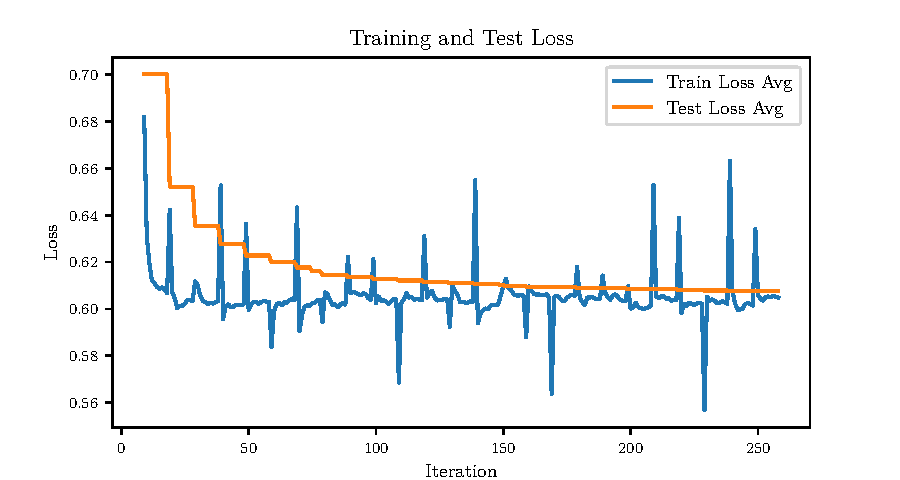
\includegraphics{img/plots/eer_finetuned_model_batch128.pdf}}
    \settoheight{\imageheight}{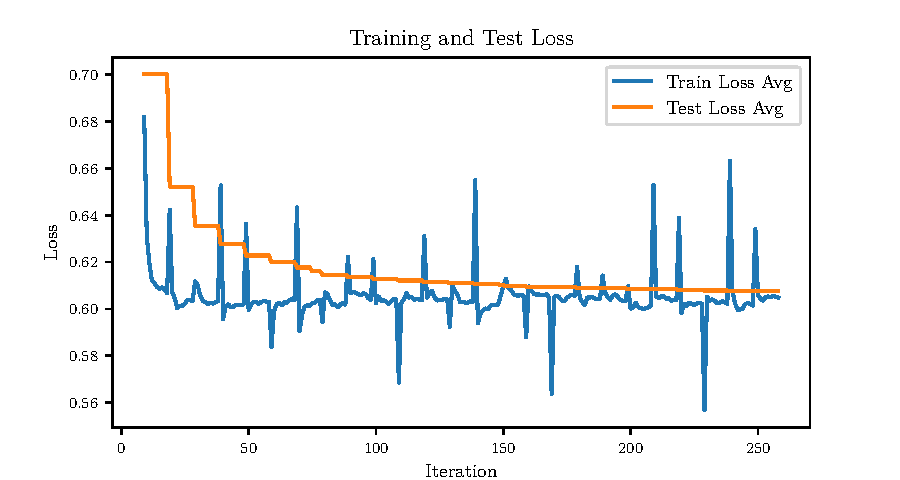
\includegraphics{img/plots/eer_finetuned_model_batch128.pdf}}
        \node[anchor=south west,inner sep=0] (image) at (0,0) {
            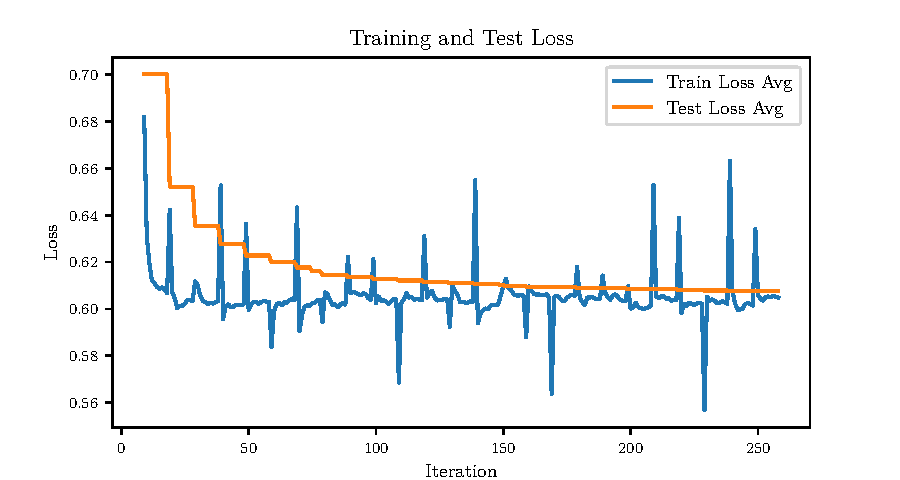
\includegraphics[width=1\linewidth, clip, viewport=0 0.0\imageheight{} \imagewidth{} 0.89\imageheight{}]{img/plots/eer_finetuned_model_batch128.pdf}
        };
    %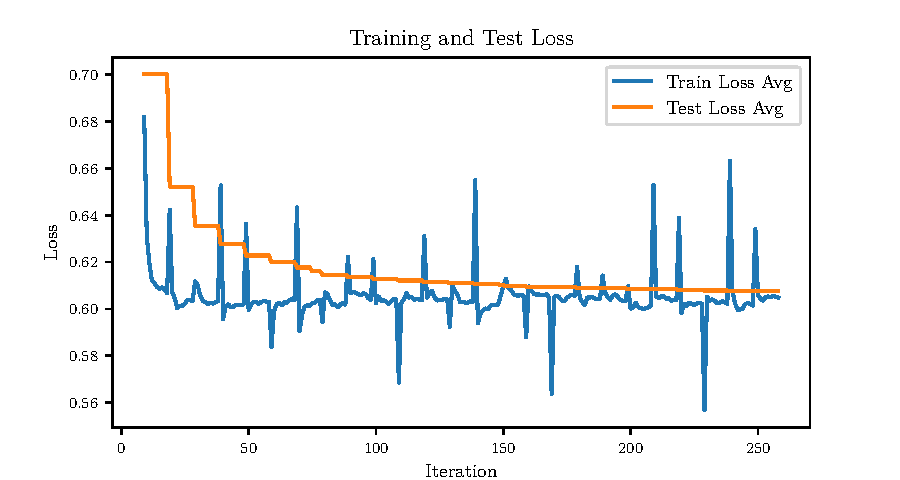
\includegraphics[width=1\linewidth]{img/plots/eer_finetuned_model_batch128.pdf}
    \end{tikzpicture}
    \caption{Training and test loss of \gls{moo} during 5 epochs.}
    \label{fig:loss:finetune}
\end{figure}


\subsection{Experiment 3}
\label{results:experiment3}

As delineated in \ref{methods_finetune_thirdAttempt}, a third experimental iteration has been conducted over the past few days preceding the submission of this thesis. The results derived from this experiment may provide additional substantiation for the hypothesis articulated in \ref{result}, specifically that transformer networks indeed possess an inductive bias towards learning \gls{sst}. Table \ref{finetuning_v3_results_transformer} corroborates that extended training duration enhances performance for \gls{sr}, yielding optimal outcomes. Additionally, the observed performance decline between original and shuffled spectrograms is significantly more pronounced than in previous results.

When evaluating the cosine similarity in table \ref{finetuning_v3_similarity_transformer}, a significant discrepancy between the positive and negative similarities indicates an improved \gls{eer}. However, the poor performance on the shuffled data is evidenced by cosine similarity values that are very close to each other.

\subsubsection{Validity of Neururer's Hypothesis}

To ascertain the validity of Neururer's hypothesis, it is imperative to train an additional model using shuffled spectrograms and assess its performance. Should it be demonstrated that a model trained on shuffled spectrograms fails to surpass the performance of the current model, this would constitute definitive evidence that transformer networks harbor an inductive bias for learning \gls{sst}. However, within the scope of this thesis, the results presented in tables \ref{finetuning_v2_results_transformer} and \ref{finetuning_v3_results_transformer} are not directly comparable.


\begin{table*}[h]
    \centering
    \caption{Test results of the finetuning using original spectrograms from the Librispeech and Voxceleb 1/2 dataset. \Gls{sr} performance is measured using the \gls{eer}. Bold font indicates best results per model, cell coloring scales with quality per model.}
        \begin{tabular}{>{\centering\arraybackslash}p{1.5cm}| >{\centering\arraybackslash}p{2.5cm} >{\centering\arraybackslash}p{2.5cm}|>{\centering\arraybackslash}p{4cm}  >{\centering\arraybackslash}p{4cm}}
            \hline
            % \multicolumn{2}{c|}{task $\rightarrow$}
            % & \multicolumn{2}{c}{\acrlong{sr}} \\
            \scriptsize{model}
            & \multicolumn{2}{c|}{\scriptsize{pretraining $\downarrow$ / finetuning $\downarrow$ / test $\rightarrow$}}
            & original
            & shuffled \\ 
            \hline
            \gls{moo}
            & original 
            & original
            & \cellcolor[RGB]{0, 255, 0} \textbf{6.54}
            & \cellcolor[RGB]{255, 0, 0} 19.61 \\
            \hline
        \end{tabular}
    \label{finetuning_v3_results_transformer}
\end{table*}


\begin{table*}[h]
    \centering
    \caption{Test results of the finetuning using original spectrograms from the Librispeech and Voxceleb 1/2 dataset. \Gls{sr} performance is measured using the cosine similarity for positive pairs and for negative pairs.}
        \begin{tabular}{>{\centering\arraybackslash}p{1.5cm}| >{\centering\arraybackslash}p{2.5cm} >{\centering\arraybackslash}p{2.5cm}|>{\centering\arraybackslash}p{4cm}  >{\centering\arraybackslash}p{4cm}}
            \hline
            % \multicolumn{2}{c|}{task $\rightarrow$}
            % & \multicolumn{2}{c}{\acrlong{sr}} \\
            \scriptsize{model}
            & \multicolumn{2}{c|}{\scriptsize{pretraining $\downarrow$ / finetuning $\downarrow$ / test $\rightarrow$}}
            & original
            & shuffled \\ 
            \hline
            \gls{moo}
            & original 
            & original
            & \cellcolor[RGB]{255, 255, 255} Pos.: 0.929 Neg.: 0.425
            & \cellcolor[RGB]{255, 255, 255} Pos.: 0.972 Neg.: 0.913 \\
            \hline
        \end{tabular}
    \label{finetuning_v3_similarity_transformer}
\end{table*}
\chapter{Conclusion}
\label{chapter:conclusion}
% 5. Conclusions
% - Summary [Summarize your thesis, including approach, results, and main knowledge gaines; brag about what you have achieved! Speculate about future]
% - Future work [short-, mid-, and long-term things one sould do; this can be a very valuable, and hence, longer, section]



\section{Summary}
In this thesis, we successfully showed that the \gls{ssast} can be used for \gls{sr}. Therefor the model described in \cite{gong2022ssast} has successfully been rebuilt, achieving the same loss and performance on the pretraining task. Additionally, a model has been pretrained on shuffled spectrograms.

These models have then been finetuned for the downstream task of \gls{sr} on the Librispeech + VoxCeleb 1/2 dataset containing speech utterances of 10 seconds from 9593 individual speakers. With these finetuned models, it was possible to further investigate the potential of transformers to learn \gls{sst}.

The finetuned models developed for this thesis did not reach state-of-the-art performance in \gls{sr}. Several factors have been identified that could improve the performance.

Nevertheless, the results of this work do show the potential of using shuffled audio data to train \gls{sr} systems. In this work, such models outperformed the models trained on original data.

\section{Future Work}

Future research should focus on several factors to improve the performance of transformers for \gls{sr} as well as the understanding of the degree to which they are able to model \gls{sst} in \gls{sr} related tasks.

\subsection{Architecture Enhancement}
Future work could benefit from experimenting with different transformer network architectures to capture temporal dependencies more effectively. Variants such as the \gls{vit} or Swin Transformer could be explored.

\subsection{Hyperparameter Tuning}
Systematic tuning of hyperparameters, including learning rate, batch size, and network architecture, is essential. Advanced techniques such as Bayesian optimization or grid search could be employed to identify optimal configurations.

\subsection{Extended Training Duration}
Increasing the training duration may allow models to reach better performance by avoiding convergence to local minima. Long-term training with regular evaluation checkpoints can provide insights into performance trends and potential improvements.

\subsection{Advanced Pooling Strategies}
Investigating different pooling strategies and dimensions for the finetuning head might yield better speaker representation embeddings. Techniques such as attention pooling or learnable pooling parameters could be tested.

\subsection{Enhanced Contrastive Learning}
Refining the contrastive learning approach, possibly through the use of larger batch sizes or more sophisticated contrastive loss functions, might lead to improved speaker representations. Hard negative mining could further improve the learning process.

By addressing these areas, future research can build upon the findings of this thesis and might find an answer to falsifiable the potential of transformer networks to learn \gls{sst}.

% % Bibliography
% \bibliographystyle{IEEEtran}
% % \bibliographystyle{unsrt}
% \bibliography{bibliography}

% \addcontentsline{toc}{chapter}{Bibliography}

% Bibliography - handled by biblatex
\printbibliography[heading=bibintoc, title={Bibliography}]


% Appendices
\appendix
% appendices


\chapter{Resynthesizing Audio from Spectrograms}
\label{appendix_resynth}




% \clearpage
% \chapter{correccted}

The \gls{ssast} is trained on Mel spectrograms, which are 2-dimensional representations of the frequencies present in an audio sample. The columns in a spectrogram are derived from the amplitude response, i.e. the absolute value of the Fourier transform (Equation \ref{eq:power_spectrum}). This process results in the loss of phase information. To resynthesize the raw audio signal from its spectrogram, the phase must be estimated, which can be done using the Griffin-Lim algorithm \cite{Griffin1983SignalEF}. Although there is no implementation for \textit{Mel} spectrograms in torchaudio, the librosa library offers this functionality in a feature inversion function called \href{https://librosa.org/doc/main/generated/librosa.feature.inverse.mel_to_audio.html}{\texttt{mel\_to\_audio}} \cite{McFee2015librosaAA}.

However, there are notable differences in the Mel spectrograms calculated by the two libraries for the same audio file. Mel spectrograms from torchaudio default to a $\log_e$ scale, which is the scale used in the original training of the \gls{ssast}. In contrast, the feature inversion function of librosa expects the spectrogram to be on a linear scale. Additionally, as described in Section \ref{sec:mel_spectrogram_conversion}, torchaudio applies a pre-emphasis filter (Equation \ref{eq:preemphasis}), but librosa does not. To mitigate these differences, a custom function, described below, was implemented.

Given a Mel spectrogram to be resynthesized, $X \in \mathbb{R}^{M \times L}$, and a reference audio signal $s_{\text{reference}} \in \mathbb{R}^l$, the function \href{https://github.com/Ironmomo/SpeakerVerificationBA/blob/master/plots_and_audios/audios_thesis.ipynb}{\texttt{synthesize\_audio\_from\_spectrogram}} performs the following operations:

First, it computes the Mel spectrogram of the reference signal $s_{\text{reference}}$ using both librosa's \href{https://librosa.org/doc/main/generated/librosa.feature.melspectrogram.html}{\texttt{melspectrogram}} function ($\rightarrow X_{\text{librosa}}$) and torchaudio's Kaldi-compliant \href{https://pytorch.org/audio/main/generated/torchaudio.compliance.kaldi.fbank.html}{\texttt{fbank}} function ($\rightarrow X_{\text{torchaudio}}$). The resulting spectrograms are then transformed to the dB scale.

Next, an additive transformation aligns the spectrogram computed by torchaudio, $X_{\text{torchaudio}}$, with that computed by librosa, $X_{\text{librosa}}$. This is achieved by adding a polynomial function $p(f)$,
\begin{equation}
    p(f) := \sum_{i=0}^{n} c_i f^i,
\end{equation}
to each frame of $X_{\text{torchaudio}}$ to minimize the difference:
\begin{equation}
   \Delta X(f, t) := X_{\text{librosa}}(f, t) - X_{\text{torchaudio}}(f, t). 
\end{equation}

The polynomial $p(f)$ is fitted by solving a least squares problem:
\begin{equation}
c = \text{argmin}_c ||\Delta X(f, t) - p(f)||^2,
\end{equation}
where $f$ is the Mel frequency bin index, $t$ is the time frame index, $n$ is the order of the polynomial, and $c_i$ are the coefficients of the polynomial.

The coefficient vector $c \in \mathbb{R}^{n+1}$ can be calculated by solving the normal equation:
\begin{equation}
A^T A c = A^T b \Rightarrow c = (A^T A)^{-1} A^T b
\end{equation}
where $A \in \mathbb{R}^{(M \cdot L) \times (n+1)}$ is the matrix of polynomial features and $b \in \mathbb{R}^{M \cdot L}$ is the (flattened) vector of differences between the two Mel spectrograms.

The polynomial $p(f)$ is then applied to the Mel spectrogram to be synthesized, $X(f, t)$, to account for the differences between the two libraries:
\begin{equation}
X_{\text{adjusted}}(f, t) = X(f, t) + p(f)
\end{equation}
Figure \ref{fig:resynthesis_adjustments} shows this process for a cross section (one frame/column) of a spectrogram.

Finally, the adjusted Mel spectrogram is transformed back to a linear scale and synthesized into audio using the feature inversion function \href{https://librosa.org/doc/main/generated/librosa.feature.inverse.mel_to_audio.html}{\texttt{mel\_to\_audio}} from the librosa library.

\begin{figure}[H]
    \centering
    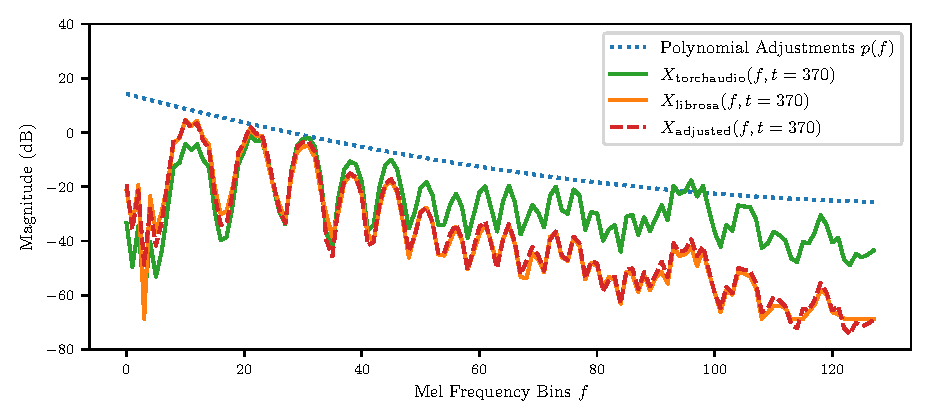
\includegraphics[width=1\linewidth]{img/plots/resynthesis_adjustments.pdf}
    \caption{Illustration of the polynomial adjustments $p(f)$ calculated from the difference between the Mel spectrograms of the reference audio signal (blue, dotted). Additionally, a cross-section of the Mel spectrograms at the $370^{\text{th}}$ time frame is shown.}
    \label{fig:resynthesis_adjustments}
\end{figure}












\clearpage
\chapter{More Resynthesized Spectrograms}\label{appendix_resynth_examples}

This appendix contains further examples of the pretrained model (trained on original data) reconstructing spectrograms. Figure \ref{fig:speech_reconstruction} and \ref{fig:music_reconstruction} contain $N=180$ manually constructed mask indices which translate to a time duration of 3.6 seconds in total. Each mask has an extent/width of 20 frame-like patches, which corresponds to 0.4 seconds of audio.

\begin{figure}[htbp]
    \centering
    \begin{tikzpicture}
        \node[anchor=south west,inner sep=0] (image) at (0,0) {
            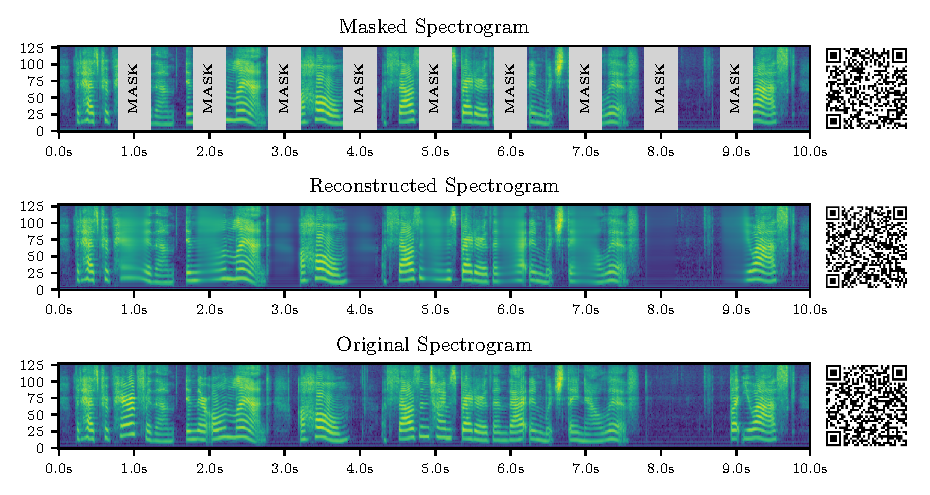
\includegraphics[width=1\linewidth]{img/plots/reconstructed_spectrogram_speech.pdf}
        };
        
        % Define the scope for the image size
        \begin{scope}[x={(image.south east)},y={(image.north west)}]
            % Define clickable areas
            \node at (0.93,0.81875) {                \href{https://github.com/Ironmomo/SpeakerVerificationBA/raw/master/plots_and_audios/audios/masked_speech.wav}{
                    \tikz{\path[fill=none] (0,0) rectangle (0.07,0.165);}
                }
            };
            \node at (0.93,0.5) {                \href{https://github.com/Ironmomo/SpeakerVerificationBA/raw/master/plots_and_audios/audios/reconstructed_speech.wav}{
                    \tikz{\path[fill=none] (0,0) rectangle (0.07,0.165);}
                }
            };
            \node at (0.93,0.18125) {                \href{https://github.com/Ironmomo/SpeakerVerificationBA/raw/master/plots_and_audios/audios/original_speech.wav}{
                    \tikz{\path[fill=none] (0,0) rectangle (0.07,0.165);}
                }
            };
        \end{scope}
    \end{tikzpicture}
    \caption{Reconstructing the same spectrogram as in Figure \ref{fig:originalModel_spectrogramReconstruction} and \ref{fig:shuffledModel_spectrogramReconstruction}, but using a manually chosen set $I$ of masked indices. Resynthesized audio files from each spectrogram can be downloaded by clicking or scanning the corresponding QR-Code.}
    \label{fig:speech_reconstruction}
\end{figure}

The sample that was used for Figure \ref{fig:speech_reconstruction} is the same that was already used in Figure \ref{fig:originalModel_spectrogramReconstruction} and \ref{fig:shuffledModel_spectrogramReconstruction}. Figure \ref{fig:music_reconstruction} shows the reconstruction of a spectrogram of music. The longest trained models (trained for 10 epochs / 428k Iterations), seems to have a quite accurate sense of melody and rhythm.

Figure \ref{fig:speech_reconstruction_longmask} shows a masked spectrogram with one large mask of 1.6 seconds at the center of the spectrogram. As can be seen in the \textit{Reconstructed Spectrogram from Original Model}, even the model trained on original spectrograms tends to make something resembling the average, if a masked patch has a large width.

% \newgeometry{top=1.0in}
\begin{figure}[h]
% \vspace{-2pt}
    \centering
    \begin{tikzpicture}
    % \settowidth{\imagewidth}{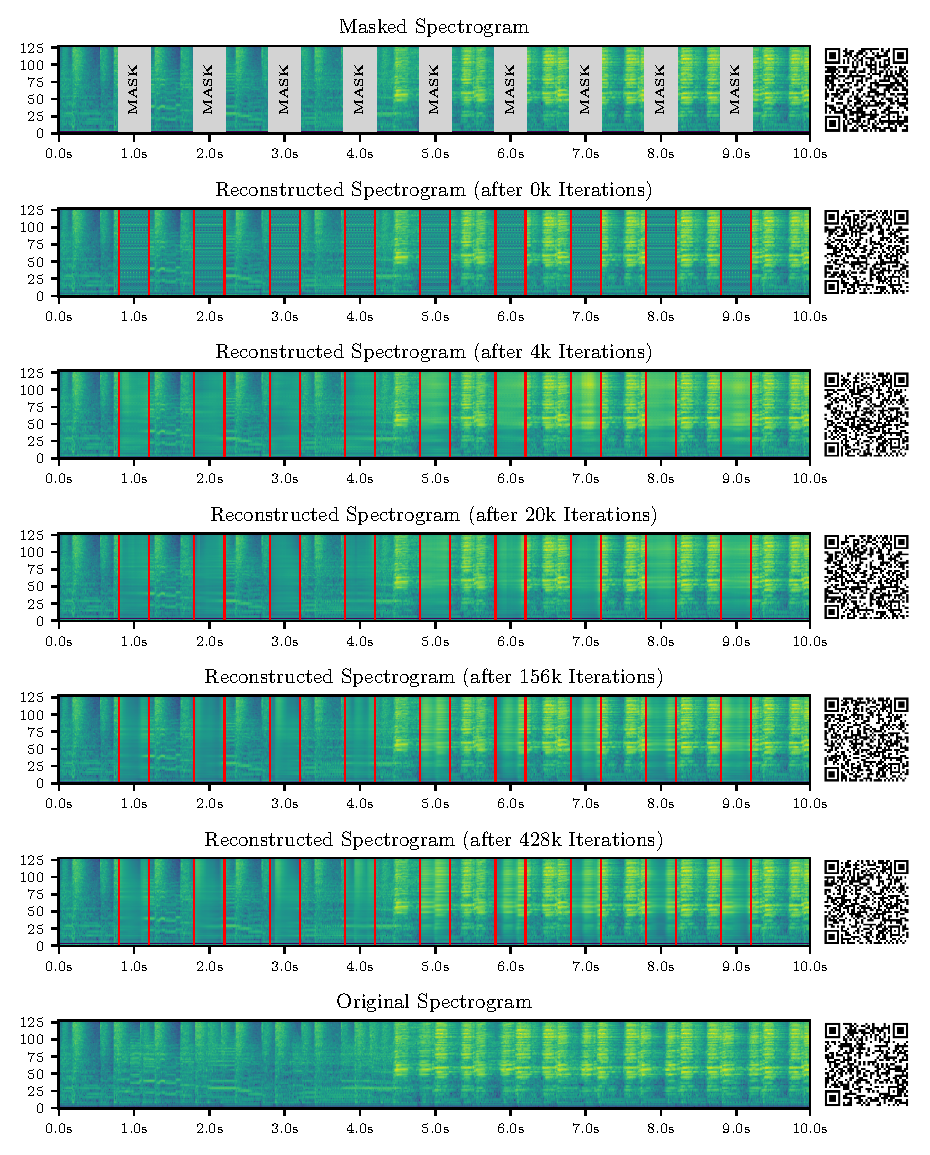
\includegraphics{img/plots/reconstructed_spectrogram_music.pdf}}
    % \settoheight{\imageheight}{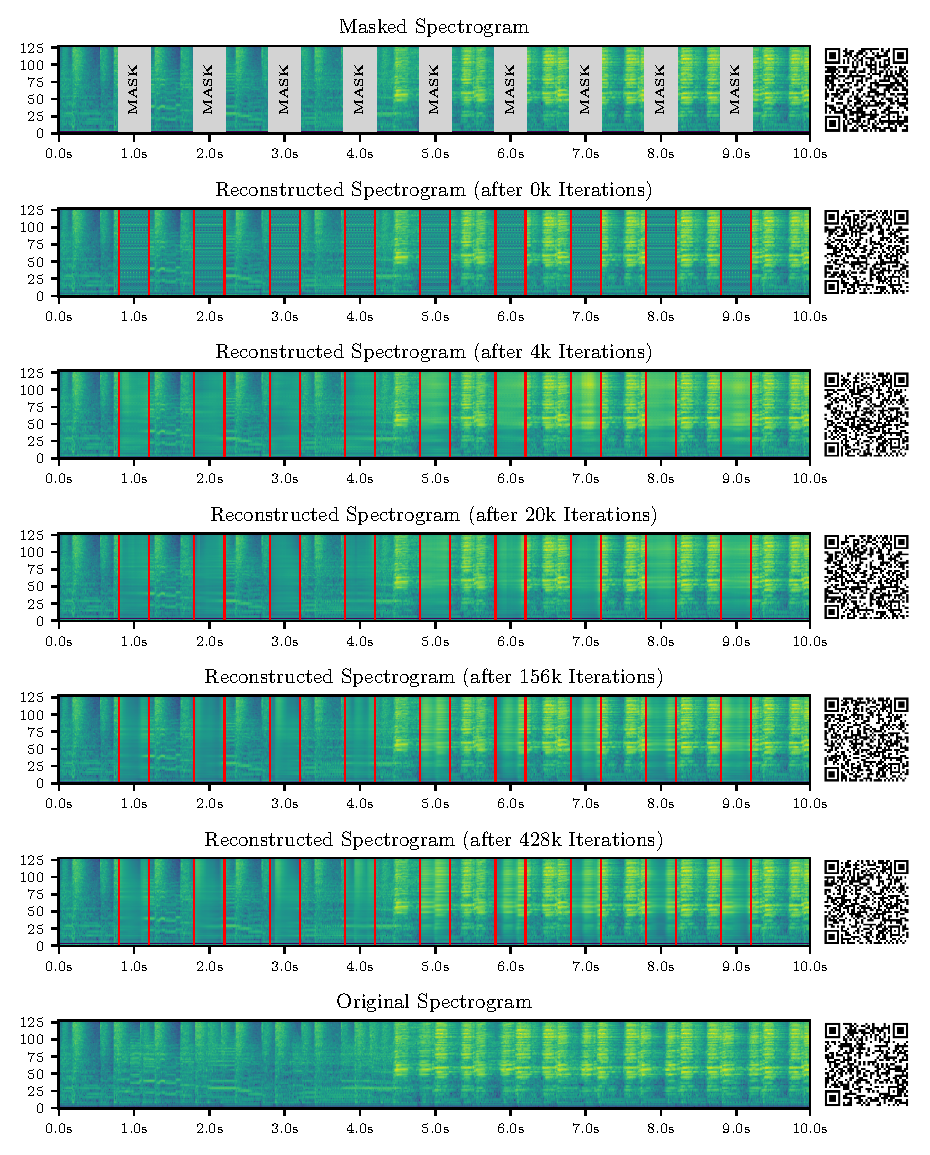
\includegraphics{img/plots/reconstructed_spectrogram_music.pdf}}
    %     \node[anchor=south west,inner sep=0] (image) at (0,0) {
    %         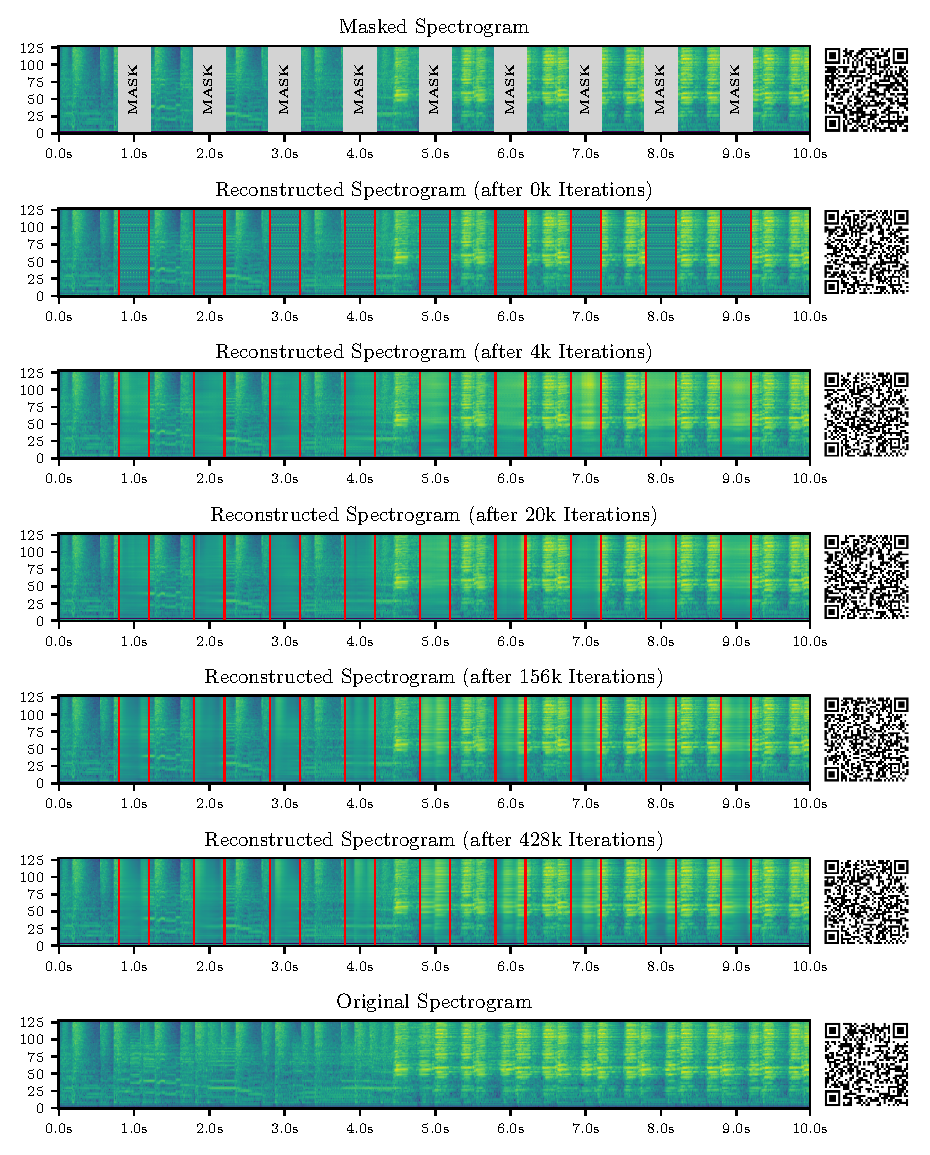
\includegraphics[width=1\linewidth, clip, viewport=0 0.01\imageheight{} \imagewidth{} 0.99\imageheight{}]{img/plots/reconstructed_spectrogram_music.pdf}
    %     };
        \node[anchor=south west,inner sep=0] (image) at (0,0) {
            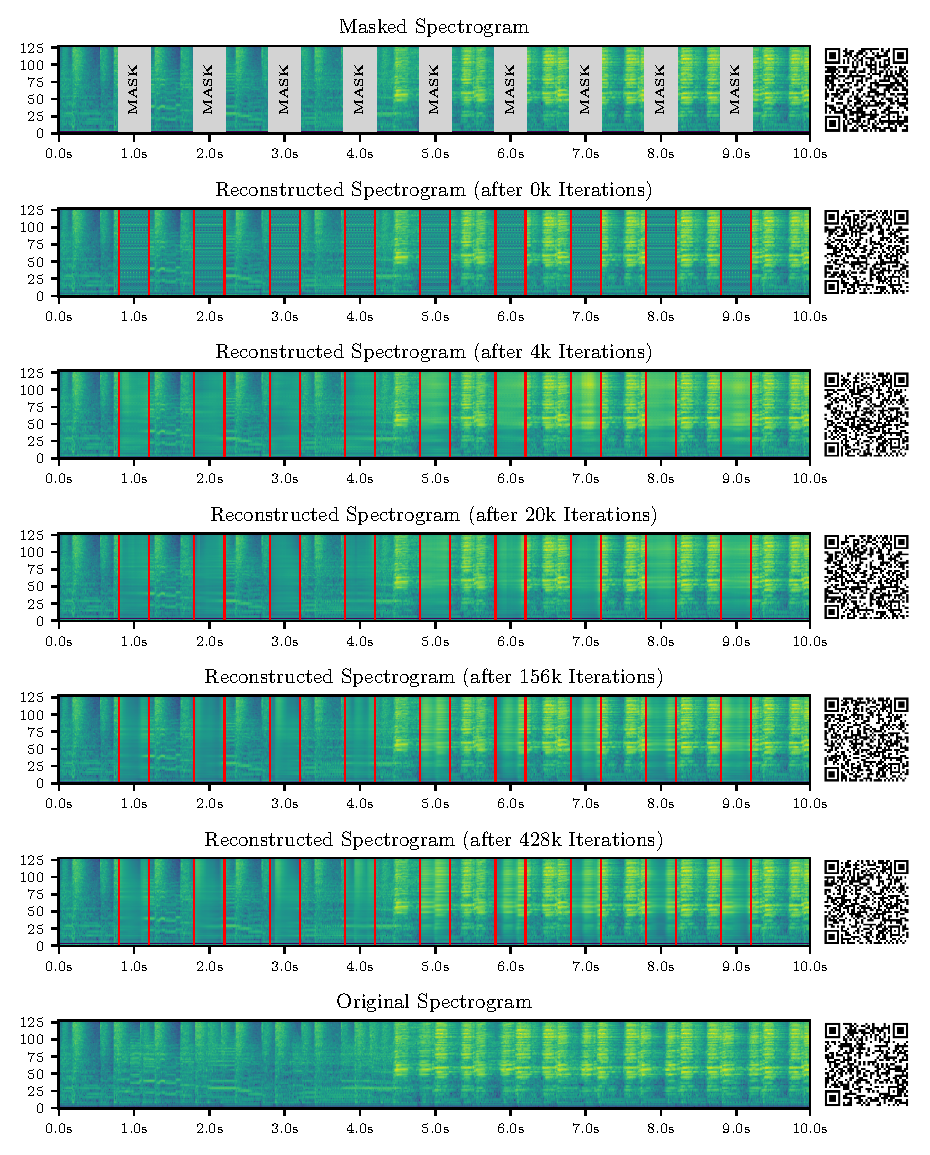
\includegraphics[width=1\linewidth]{img/plots/reconstructed_spectrogram_music.pdf}
        };
        
        % Define the scope for the image size
        \begin{scope}[x={(image.south east)},y={(image.north west)}]
            % Define clickable areas
            \node at (0.93,0.08+6.0/7.1) {                \href{https://github.com/Ironmomo/SpeakerVerificationBA/raw/master/plots_and_audios/audios/masked_music.wav}{
                    \tikz{\path[fill=none] (0,0) rectangle (0.07,0.07);} % (x, y) ≙ (width, height)
                }
            };
            \node at (0.93,0.08+5.0/7.1) {                \href{https://github.com/Ironmomo/SpeakerVerificationBA/raw/master/plots_and_audios/audios/reconstructed_music_1.wav}{
                    \tikz{\path[fill=none] (0,0) rectangle (0.07,0.07);}
                }
            };
            \node at (0.93,0.08+4.0/7.1) {                \href{https://github.com/Ironmomo/SpeakerVerificationBA/raw/master/plots_and_audios/audios/reconstructed_music_2.wav}{
                    \tikz{\path[fill=none] (0,0) rectangle (0.07,0.07);}
                }
            };
            \node at (0.93,0.08+3.0/7.1) {                \href{https://github.com/Ironmomo/SpeakerVerificationBA/raw/master/plots_and_audios/audios/reconstructed_music_6.wav}{
                    \tikz{\path[fill=none] (0,0) rectangle (0.07,0.07);}
                }
            };
            \node at (0.93,0.08+2.0/7.1) {                \href{https://github.com/Ironmomo/SpeakerVerificationBA/raw/master/plots_and_audios/audios/reconstructed_music_40.wav}{
                    \tikz{\path[fill=none] (0,0) rectangle (0.07,0.07);}
                }
            };
            \node at (0.93,0.08+1.0/7.1) {                \href{https://github.com/Ironmomo/SpeakerVerificationBA/raw/master/plots_and_audios/audios/reconstructed_music_108.wav}{
                    \tikz{\path[fill=none] (0,0) rectangle (0.07,0.07);}
                }
            };
            \node at (0.93,0.08) {                \href{https://github.com/Ironmomo/SpeakerVerificationBA/raw/master/plots_and_audios/audios/original_music.wav}{
                    \tikz{\path[fill=none] (0,0) rectangle (0.07,0.07);}
                }
            };
        \end{scope}
    \end{tikzpicture}
    % \captionsetup{aboveskip=0pt, belowskip=-55pt}
    \caption{Reconstructing a spectrogram of music with the model at different stages of pretraining. Resynthesized audio files from each spectrogram can be downloaded by clicking or scanning the corresponding QR-Code.}
    \label{fig:music_reconstruction}
\end{figure}
\clearpage
% \restoregeometry



\begin{figure}[htbp]
    \centering
    \begin{tikzpicture}
        \node[anchor=south west,inner sep=0] (image) at (0,0) {
            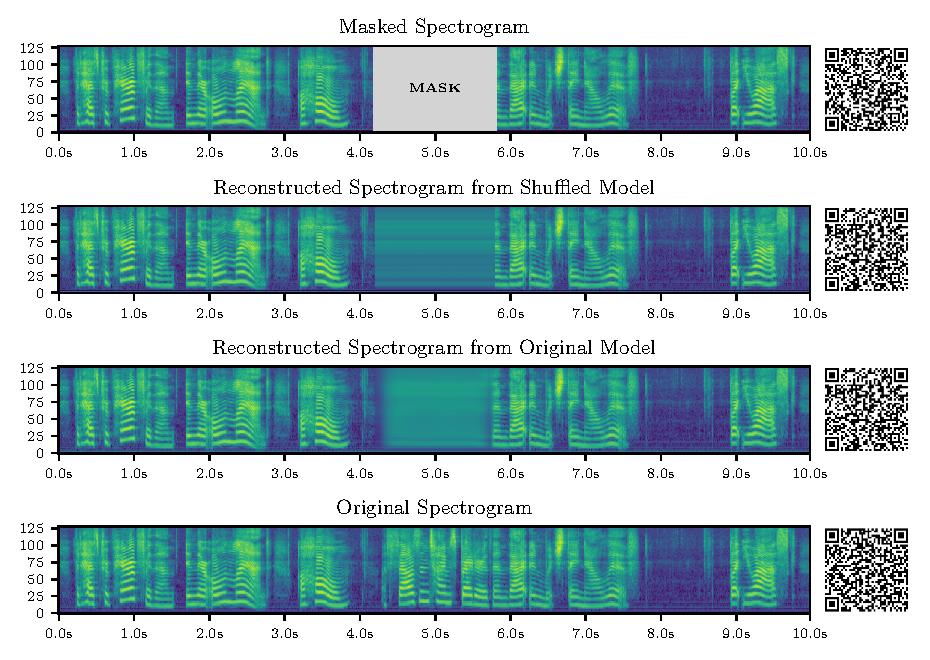
\includegraphics[width=1\linewidth]{img/plots/reconstructed_spectrogram_speech_longmask.pdf}
        };
        
        % Define the scope for the image size
        \begin{scope}[x={(image.south east)},y={(image.north west)}]
            % Define clickable areas
            \node at (0.93,0.138+3*0.242) {                \href{https://github.com/Ironmomo/SpeakerVerificationBA/raw/master/plots_and_audios/audios/masked_speech_longmask.wav}{
                    \tikz{\path[fill=none] (0,0) rectangle (0.07,0.12);}
                }
            };
            \node at (0.93,0.138+2*0.242) {                \href{https://github.com/Ironmomo/SpeakerVerificationBA/raw/master/plots_and_audios/audios/reconstructed_speech_SUModel_longmask.wav}{
                    \tikz{\path[fill=none] (0,0) rectangle (0.07,0.12);}
                }
            };
            \node at (0.93,0.138+0.242) {                \href{https://github.com/Ironmomo/SpeakerVerificationBA/raw/master/plots_and_audios/audios/reconstructed_speech_OSModel_longmask.wav}{
                    \tikz{\path[fill=none] (0,0) rectangle (0.07,0.12);}
                }
            };
            \node at (0.93,0.138) {                \href{https://github.com/Ironmomo/SpeakerVerificationBA/raw/master/plots_and_audios/audios/original_speech.wav}{
                    \tikz{\path[fill=none] (0,0) rectangle (0.07,0.12);}
                }
            };
        \end{scope}
    \end{tikzpicture}
    \caption{Manually masking $N=80$ of the frame-like $2 \times 128$ patches, but aligning the masks all at the center and next to each other, forming one large mask of 1.6 seconds. Resynthesized audio files from each spectrogram can be downloaded by clicking or scanning the corresponding QR-Code.}
    \label{fig:speech_reconstruction_longmask}
\end{figure}


\end{document}
